\documentclass[twoside]{book}

% Packages required by doxygen
\usepackage{fixltx2e}
\usepackage{calc}
\usepackage{doxygen}
\usepackage[export]{adjustbox} % also loads graphicx
\usepackage{graphicx}
\usepackage[utf8]{inputenc}
\usepackage{makeidx}
\usepackage{multicol}
\usepackage{multirow}
\PassOptionsToPackage{warn}{textcomp}
\usepackage{textcomp}
\usepackage[nointegrals]{wasysym}
\usepackage[table]{xcolor}

% Font selection
\usepackage[T1]{fontenc}
\usepackage[scaled=.90]{helvet}
\usepackage{courier}
\usepackage{amssymb}
\usepackage{sectsty}
\renewcommand{\familydefault}{\sfdefault}
\allsectionsfont{%
  \fontseries{bc}\selectfont%
  \color{darkgray}%
}
\renewcommand{\DoxyLabelFont}{%
  \fontseries{bc}\selectfont%
  \color{darkgray}%
}
\newcommand{\+}{\discretionary{\mbox{\scriptsize$\hookleftarrow$}}{}{}}

% Page & text layout
\usepackage{geometry}
\geometry{%
  a4paper,%
  top=2.5cm,%
  bottom=2.5cm,%
  left=2.5cm,%
  right=2.5cm%
}
\tolerance=750
\hfuzz=15pt
\hbadness=750
\setlength{\emergencystretch}{15pt}
\setlength{\parindent}{0cm}
\setlength{\parskip}{3ex plus 2ex minus 2ex}
\makeatletter
\renewcommand{\paragraph}{%
  \@startsection{paragraph}{4}{0ex}{-1.0ex}{1.0ex}{%
    \normalfont\normalsize\bfseries\SS@parafont%
  }%
}
\renewcommand{\subparagraph}{%
  \@startsection{subparagraph}{5}{0ex}{-1.0ex}{1.0ex}{%
    \normalfont\normalsize\bfseries\SS@subparafont%
  }%
}
\makeatother

% Headers & footers
\usepackage{fancyhdr}
\pagestyle{fancyplain}
\fancyhead[LE]{\fancyplain{}{\bfseries\thepage}}
\fancyhead[CE]{\fancyplain{}{}}
\fancyhead[RE]{\fancyplain{}{\bfseries\leftmark}}
\fancyhead[LO]{\fancyplain{}{\bfseries\rightmark}}
\fancyhead[CO]{\fancyplain{}{}}
\fancyhead[RO]{\fancyplain{}{\bfseries\thepage}}
\fancyfoot[LE]{\fancyplain{}{}}
\fancyfoot[CE]{\fancyplain{}{}}
\fancyfoot[RE]{\fancyplain{}{\bfseries\scriptsize Generated by Doxygen }}
\fancyfoot[LO]{\fancyplain{}{\bfseries\scriptsize Generated by Doxygen }}
\fancyfoot[CO]{\fancyplain{}{}}
\fancyfoot[RO]{\fancyplain{}{}}
\renewcommand{\footrulewidth}{0.4pt}
\renewcommand{\chaptermark}[1]{%
  \markboth{#1}{}%
}
\renewcommand{\sectionmark}[1]{%
  \markright{\thesection\ #1}%
}

% Indices & bibliography
\usepackage{natbib}
\usepackage[titles]{tocloft}
\setcounter{tocdepth}{3}
\setcounter{secnumdepth}{5}
\makeindex

% Hyperlinks (required, but should be loaded last)
\usepackage{ifpdf}
\ifpdf
  \usepackage[pdftex,pagebackref=true]{hyperref}
\else
  \usepackage[ps2pdf,pagebackref=true]{hyperref}
\fi
\hypersetup{%
  colorlinks=true,%
  linkcolor=blue,%
  citecolor=blue,%
  unicode%
}

% Custom commands
\newcommand{\clearemptydoublepage}{%
  \newpage{\pagestyle{empty}\cleardoublepage}%
}

\usepackage{caption}
\captionsetup{labelsep=space,justification=centering,font={bf},singlelinecheck=off,skip=4pt,position=top}

%===== C O N T E N T S =====

\begin{document}

% Titlepage & ToC
\hypersetup{pageanchor=false,
             bookmarksnumbered=true,
             pdfencoding=unicode
            }
\pagenumbering{alph}
\begin{titlepage}
\vspace*{7cm}
\begin{center}%
{\Large V\+H\+DL calculator project B\+E\+L3 }\\
\vspace*{1cm}
{\large Generated by Doxygen 1.8.13}\\
\end{center}
\end{titlepage}
\clearemptydoublepage
\pagenumbering{roman}
\tableofcontents
\clearemptydoublepage
\pagenumbering{arabic}
\hypersetup{pageanchor=true}

%--- Begin generated contents ---
\chapter{Design Unit Index}
\section{Design Unit Hierarchy}
This inheritance list is sorted roughly, but not completely, alphabetically\+:\begin{DoxyCompactList}
\item \contentsline{section}{tb\+\_\+alu}{\pageref{classtb__alu}}{}
\begin{DoxyCompactList}
\item \contentsline{section}{alu}{\pageref{classalu}}{}
\end{DoxyCompactList}
\item \contentsline{section}{tb\+\_\+calc\+\_\+ctrl}{\pageref{classtb__calc__ctrl}}{}
\begin{DoxyCompactList}
\item \contentsline{section}{calc\+\_\+ctrl}{\pageref{classcalc__ctrl}}{}
\end{DoxyCompactList}
\item \contentsline{section}{tb\+\_\+calc\+\_\+top}{\pageref{classtb__calc__top}}{}
\begin{DoxyCompactList}
\item \contentsline{section}{calc\+\_\+top}{\pageref{classcalc__top}}{}
\begin{DoxyCompactList}
\item \contentsline{section}{io\+\_\+ctrl}{\pageref{classio__ctrl}}{}
\item \contentsline{section}{calc\+\_\+ctrl}{\pageref{classcalc__ctrl}}{}
\item \contentsline{section}{alu}{\pageref{classalu}}{}
\end{DoxyCompactList}
\end{DoxyCompactList}
\item \contentsline{section}{tb\+\_\+io\+\_\+ctrl}{\pageref{classtb__io__ctrl}}{}
\begin{DoxyCompactList}
\item \contentsline{section}{io\+\_\+ctrl}{\pageref{classio__ctrl}}{}
\end{DoxyCompactList}
\end{DoxyCompactList}

\chapter{Design Unit Index}
\section{Design Unit List}
Here is a list of all design unit members with links to the Entities they belong to\+:\begin{DoxyCompactList}
\item\contentsline{section}{entity \hyperlink{classalu}{alu} \\*A\+LU Entity }{\pageref{classalu}}{}
\item\contentsline{section}{entity \hyperlink{classcalc__ctrl}{calc\+\_\+ctrl} \\*Calculator Control Unit Entity }{\pageref{classcalc__ctrl}}{}
\item\contentsline{section}{entity \hyperlink{classcalc__top}{calc\+\_\+top} \\*Calculator Top Design Entity }{\pageref{classcalc__top}}{}
\item\contentsline{section}{entity \hyperlink{classio__ctrl}{io\+\_\+ctrl} \\*IO Control Unit Entity }{\pageref{classio__ctrl}}{}
\item\contentsline{section}{architecture \hyperlink{classio__ctrl_1_1rtl}{rtl} \\*IO Control Unit Architecture R\+TL }{\pageref{classio__ctrl_1_1rtl}}{}
\item\contentsline{section}{architecture \hyperlink{classalu_1_1rtl}{rtl} \\*A\+LU Architecture R\+TL }{\pageref{classalu_1_1rtl}}{}
\item\contentsline{section}{architecture \hyperlink{classcalc__ctrl_1_1rtl}{rtl} \\*Calclator Control Unit Architecture R\+TL }{\pageref{classcalc__ctrl_1_1rtl}}{}
\item\contentsline{section}{architecture \hyperlink{classtb__calc__ctrl_1_1sim}{sim} \\*Calculcator Control Unit Testbench Architecture S\+IM }{\pageref{classtb__calc__ctrl_1_1sim}}{}
\item\contentsline{section}{architecture \hyperlink{classtb__io__ctrl_1_1sim}{sim} \\*IO Control Unit Testbench Architecture S\+IM }{\pageref{classtb__io__ctrl_1_1sim}}{}
\item\contentsline{section}{architecture \hyperlink{classtb__alu_1_1sim}{sim} \\*A\+LU Testbench Architecture S\+IM }{\pageref{classtb__alu_1_1sim}}{}
\item\contentsline{section}{architecture \hyperlink{classtb__calc__top_1_1sim}{sim} \\*Calculator Top Design Testbench Architecture S\+IM }{\pageref{classtb__calc__top_1_1sim}}{}
\item\contentsline{section}{architecture \hyperlink{classcalc__top_1_1struc}{struc} \\*Calculator Top Architecture R\+T\+L-\/\+S\+T\+R\+UC }{\pageref{classcalc__top_1_1struc}}{}
\item\contentsline{section}{entity \hyperlink{classtb__alu}{tb\+\_\+alu} \\*A\+LU Testbench Entity }{\pageref{classtb__alu}}{}
\item\contentsline{section}{entity \hyperlink{classtb__calc__ctrl}{tb\+\_\+calc\+\_\+ctrl} \\*Calculator Control Unit Testbench Entity }{\pageref{classtb__calc__ctrl}}{}
\item\contentsline{section}{entity \hyperlink{classtb__calc__top}{tb\+\_\+calc\+\_\+top} \\*Calculator Top Design Testbench Entity }{\pageref{classtb__calc__top}}{}
\item\contentsline{section}{entity \hyperlink{classtb__io__ctrl}{tb\+\_\+io\+\_\+ctrl} \\*IO Control Unit Testbench Entity }{\pageref{classtb__io__ctrl}}{}
\end{DoxyCompactList}

\chapter{File Index}
\section{File List}
Here is a list of all documented files with brief descriptions\+:\begin{DoxyCompactList}
\item\contentsline{section}{tb/\hyperlink{tb__io__ctrl___8vhd}{tb\+\_\+io\+\_\+ctrl\+\_\+.\+vhd} \\*IO Control Unit Testbench Entity }{\pageref{tb__io__ctrl___8vhd}}{}
\item\contentsline{section}{tb/\hyperlink{tb__io__ctrl__cfg_8vhd}{tb\+\_\+io\+\_\+ctrl\+\_\+cfg.\+vhd} \\*IO Control Unit Testbench Configuration }{\pageref{tb__io__ctrl__cfg_8vhd}}{}
\item\contentsline{section}{tb/\hyperlink{tb__io__ctrl__sim_8vhd}{tb\+\_\+io\+\_\+ctrl\+\_\+sim.\+vhd} \\*IO Control Unit Testbench Architecture }{\pageref{tb__io__ctrl__sim_8vhd}}{}
\item\contentsline{section}{vhdl/\hyperlink{io__ctrl___8vhd}{io\+\_\+ctrl\+\_\+.\+vhd} \\*IO Control Unit Entity }{\pageref{io__ctrl___8vhd}}{}
\item\contentsline{section}{vhdl/\hyperlink{io__ctrl__cfg_8vhd}{io\+\_\+ctrl\+\_\+cfg.\+vhd} \\*IO Control Unit Configuration }{\pageref{io__ctrl__cfg_8vhd}}{}
\item\contentsline{section}{vhdl/\hyperlink{io__ctrl__rtl_8vhd}{io\+\_\+ctrl\+\_\+rtl.\+vhd} \\*IO Control Unit Architecture }{\pageref{io__ctrl__rtl_8vhd}}{}
\end{DoxyCompactList}

\chapter{Class Documentation}
\hypertarget{classio__ctrl}{}\section{io\+\_\+ctrl Entity Reference}
\label{classio__ctrl}\index{io\+\_\+ctrl@{io\+\_\+ctrl}}


IO Control Unit Entity.  


Inheritance diagram for io\+\_\+ctrl\+:\begin{figure}[H]
\begin{center}
\leavevmode
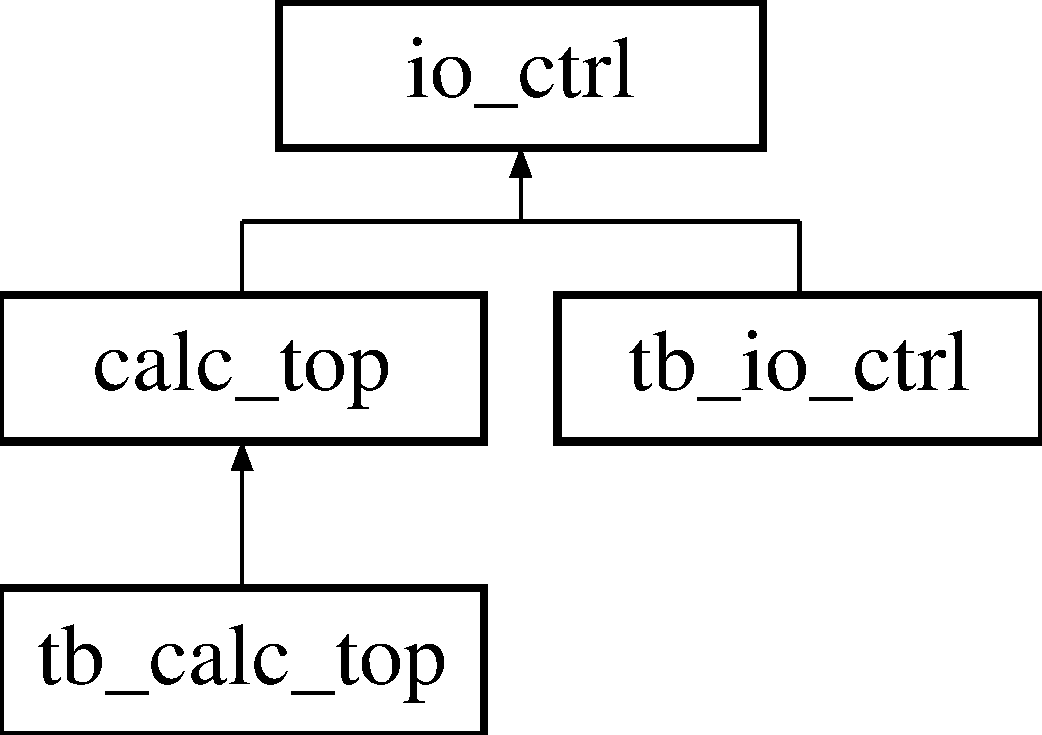
\includegraphics[height=3.000000cm]{classio__ctrl}
\end{center}
\end{figure}
\subsection*{Entities}
\begin{DoxyCompactItemize}
\item 
\hyperlink{classio__ctrl_1_1rtl}{rtl} architecture
\begin{DoxyCompactList}\small\item\em IO Control Unit Architecture R\+TL. \end{DoxyCompactList}\end{DoxyCompactItemize}
\subsection*{Libraries}
 \begin{DoxyCompactItemize}
\item 
\hyperlink{classio__ctrl_ae4f03c286607f3181e16b9aa12d0c6d4}{I\+E\+EE} 
\end{DoxyCompactItemize}
\subsection*{Use Clauses}
 \begin{DoxyCompactItemize}
\item 
\hyperlink{classio__ctrl_acd03516902501cd1c7296a98e22c6fcb}{std\+\_\+logic\+\_\+1164}   
\end{DoxyCompactItemize}
\subsection*{Ports}
 \begin{DoxyCompactItemize}
\item 
\hyperlink{classio__ctrl_abe949478e3f8aad0a6aeb1842fa6c608}{clk\+\_\+i}  {\bfseries {\bfseries \textcolor{keywordflow}{in}\textcolor{vhdlchar}{ }}} {\bfseries \textcolor{comment}{std\+\_\+logic}\textcolor{vhdlchar}{ }} 
\item 
\hyperlink{classio__ctrl_a55da7e76960757f8c6842e86a28ee7be}{reset\+\_\+i}  {\bfseries {\bfseries \textcolor{keywordflow}{in}\textcolor{vhdlchar}{ }}} {\bfseries \textcolor{comment}{std\+\_\+logic}\textcolor{vhdlchar}{ }} 
\item 
\hyperlink{classio__ctrl_a32bd80898d1d7c2a543b82a1d6ad1e6c}{dig0\+\_\+i}  {\bfseries {\bfseries \textcolor{keywordflow}{in}\textcolor{vhdlchar}{ }}} {\bfseries \textcolor{comment}{std\+\_\+logic\+\_\+vector}\textcolor{vhdlchar}{ }\textcolor{vhdlchar}{(}\textcolor{vhdlchar}{ }\textcolor{vhdlchar}{ } \textcolor{vhdldigit}{7} \textcolor{vhdlchar}{ }\textcolor{keywordflow}{downto}\textcolor{vhdlchar}{ }\textcolor{vhdlchar}{ } \textcolor{vhdldigit}{0} \textcolor{vhdlchar}{ }\textcolor{vhdlchar}{)}\textcolor{vhdlchar}{ }} 
\item 
\hyperlink{classio__ctrl_a5038eac0f38fc173af3ff10434e90921}{dig1\+\_\+i}  {\bfseries {\bfseries \textcolor{keywordflow}{in}\textcolor{vhdlchar}{ }}} {\bfseries \textcolor{comment}{std\+\_\+logic\+\_\+vector}\textcolor{vhdlchar}{ }\textcolor{vhdlchar}{(}\textcolor{vhdlchar}{ }\textcolor{vhdlchar}{ } \textcolor{vhdldigit}{7} \textcolor{vhdlchar}{ }\textcolor{keywordflow}{downto}\textcolor{vhdlchar}{ }\textcolor{vhdlchar}{ } \textcolor{vhdldigit}{0} \textcolor{vhdlchar}{ }\textcolor{vhdlchar}{)}\textcolor{vhdlchar}{ }} 
\item 
\hyperlink{classio__ctrl_a1edaf350ab71f6c0e97ba7a82c4bd16f}{dig2\+\_\+i}  {\bfseries {\bfseries \textcolor{keywordflow}{in}\textcolor{vhdlchar}{ }}} {\bfseries \textcolor{comment}{std\+\_\+logic\+\_\+vector}\textcolor{vhdlchar}{ }\textcolor{vhdlchar}{(}\textcolor{vhdlchar}{ }\textcolor{vhdlchar}{ } \textcolor{vhdldigit}{7} \textcolor{vhdlchar}{ }\textcolor{keywordflow}{downto}\textcolor{vhdlchar}{ }\textcolor{vhdlchar}{ } \textcolor{vhdldigit}{0} \textcolor{vhdlchar}{ }\textcolor{vhdlchar}{)}\textcolor{vhdlchar}{ }} 
\item 
\hyperlink{classio__ctrl_ab98d2879f1ba46721cdc9015e3f88d50}{dig3\+\_\+i}  {\bfseries {\bfseries \textcolor{keywordflow}{in}\textcolor{vhdlchar}{ }}} {\bfseries \textcolor{comment}{std\+\_\+logic\+\_\+vector}\textcolor{vhdlchar}{ }\textcolor{vhdlchar}{(}\textcolor{vhdlchar}{ }\textcolor{vhdlchar}{ } \textcolor{vhdldigit}{7} \textcolor{vhdlchar}{ }\textcolor{keywordflow}{downto}\textcolor{vhdlchar}{ }\textcolor{vhdlchar}{ } \textcolor{vhdldigit}{0} \textcolor{vhdlchar}{ }\textcolor{vhdlchar}{)}\textcolor{vhdlchar}{ }} 
\item 
\hyperlink{classio__ctrl_a7693929621a7c94dd62fd7b39db30b50}{led\+\_\+i}  {\bfseries {\bfseries \textcolor{keywordflow}{in}\textcolor{vhdlchar}{ }}} {\bfseries \textcolor{comment}{std\+\_\+logic\+\_\+vector}\textcolor{vhdlchar}{ }\textcolor{vhdlchar}{(}\textcolor{vhdlchar}{ }\textcolor{vhdlchar}{ } \textcolor{vhdldigit}{15} \textcolor{vhdlchar}{ }\textcolor{keywordflow}{downto}\textcolor{vhdlchar}{ }\textcolor{vhdlchar}{ } \textcolor{vhdldigit}{0} \textcolor{vhdlchar}{ }\textcolor{vhdlchar}{)}\textcolor{vhdlchar}{ }} 
\item 
\hyperlink{classio__ctrl_a91628ae1b8a6c62fdd738bc70aba3f1e}{sw\+\_\+i}  {\bfseries {\bfseries \textcolor{keywordflow}{in}\textcolor{vhdlchar}{ }}} {\bfseries \textcolor{comment}{std\+\_\+logic\+\_\+vector}\textcolor{vhdlchar}{ }\textcolor{vhdlchar}{(}\textcolor{vhdlchar}{ }\textcolor{vhdlchar}{ } \textcolor{vhdldigit}{15} \textcolor{vhdlchar}{ }\textcolor{keywordflow}{downto}\textcolor{vhdlchar}{ }\textcolor{vhdlchar}{ } \textcolor{vhdldigit}{0} \textcolor{vhdlchar}{ }\textcolor{vhdlchar}{)}\textcolor{vhdlchar}{ }} 
\item 
\hyperlink{classio__ctrl_ae54d0166fc1acf3023764d9869477e8b}{pb\+\_\+i}  {\bfseries {\bfseries \textcolor{keywordflow}{in}\textcolor{vhdlchar}{ }}} {\bfseries \textcolor{comment}{std\+\_\+logic\+\_\+vector}\textcolor{vhdlchar}{ }\textcolor{vhdlchar}{(}\textcolor{vhdlchar}{ }\textcolor{vhdlchar}{ } \textcolor{vhdldigit}{3} \textcolor{vhdlchar}{ }\textcolor{keywordflow}{downto}\textcolor{vhdlchar}{ }\textcolor{vhdlchar}{ } \textcolor{vhdldigit}{0} \textcolor{vhdlchar}{ }\textcolor{vhdlchar}{)}\textcolor{vhdlchar}{ }} 
\item 
\hyperlink{classio__ctrl_a818bce4de706b73d1b0168e689b5301b}{ss\+\_\+o}  {\bfseries {\bfseries \textcolor{keywordflow}{out}\textcolor{vhdlchar}{ }}} {\bfseries \textcolor{comment}{std\+\_\+logic\+\_\+vector}\textcolor{vhdlchar}{ }\textcolor{vhdlchar}{(}\textcolor{vhdlchar}{ }\textcolor{vhdlchar}{ } \textcolor{vhdldigit}{7} \textcolor{vhdlchar}{ }\textcolor{keywordflow}{downto}\textcolor{vhdlchar}{ }\textcolor{vhdlchar}{ } \textcolor{vhdldigit}{0} \textcolor{vhdlchar}{ }\textcolor{vhdlchar}{)}\textcolor{vhdlchar}{ }} 
\item 
\hyperlink{classio__ctrl_a58671df81269968cc647f9f2335477e9}{ss\+\_\+sel\+\_\+o}  {\bfseries {\bfseries \textcolor{keywordflow}{out}\textcolor{vhdlchar}{ }}} {\bfseries \textcolor{comment}{std\+\_\+logic\+\_\+vector}\textcolor{vhdlchar}{ }\textcolor{vhdlchar}{(}\textcolor{vhdlchar}{ }\textcolor{vhdlchar}{ } \textcolor{vhdldigit}{3} \textcolor{vhdlchar}{ }\textcolor{keywordflow}{downto}\textcolor{vhdlchar}{ }\textcolor{vhdlchar}{ } \textcolor{vhdldigit}{0} \textcolor{vhdlchar}{ }\textcolor{vhdlchar}{)}\textcolor{vhdlchar}{ }} 
\item 
\hyperlink{classio__ctrl_ae622b8b55ca985e4965d79aab895a746}{led\+\_\+o}  {\bfseries {\bfseries \textcolor{keywordflow}{out}\textcolor{vhdlchar}{ }}} {\bfseries \textcolor{comment}{std\+\_\+logic\+\_\+vector}\textcolor{vhdlchar}{ }\textcolor{vhdlchar}{(}\textcolor{vhdlchar}{ }\textcolor{vhdlchar}{ } \textcolor{vhdldigit}{15} \textcolor{vhdlchar}{ }\textcolor{keywordflow}{downto}\textcolor{vhdlchar}{ }\textcolor{vhdlchar}{ } \textcolor{vhdldigit}{0} \textcolor{vhdlchar}{ }\textcolor{vhdlchar}{)}\textcolor{vhdlchar}{ }} 
\item 
\hyperlink{classio__ctrl_a0d67cc1091d658566c78f05fa744f4a0}{swsync\+\_\+o}  {\bfseries {\bfseries \textcolor{keywordflow}{out}\textcolor{vhdlchar}{ }}} {\bfseries \textcolor{comment}{std\+\_\+logic\+\_\+vector}\textcolor{vhdlchar}{ }\textcolor{vhdlchar}{(}\textcolor{vhdlchar}{ }\textcolor{vhdlchar}{ } \textcolor{vhdldigit}{15} \textcolor{vhdlchar}{ }\textcolor{keywordflow}{downto}\textcolor{vhdlchar}{ }\textcolor{vhdlchar}{ } \textcolor{vhdldigit}{0} \textcolor{vhdlchar}{ }\textcolor{vhdlchar}{)}\textcolor{vhdlchar}{ }} 
\item 
\hyperlink{classio__ctrl_a95d4164acb4876609c3ee30095deba32}{pbsync\+\_\+o}  {\bfseries {\bfseries \textcolor{keywordflow}{out}\textcolor{vhdlchar}{ }}} {\bfseries \textcolor{comment}{std\+\_\+logic\+\_\+vector}\textcolor{vhdlchar}{ }\textcolor{vhdlchar}{(}\textcolor{vhdlchar}{ }\textcolor{vhdlchar}{ } \textcolor{vhdldigit}{3} \textcolor{vhdlchar}{ }\textcolor{keywordflow}{downto}\textcolor{vhdlchar}{ }\textcolor{vhdlchar}{ } \textcolor{vhdldigit}{0} \textcolor{vhdlchar}{ }\textcolor{vhdlchar}{)}\textcolor{vhdlchar}{ }} 
\end{DoxyCompactItemize}


\subsection{Detailed Description}
IO Control Unit Entity. 

The IO Control unit is part of the calculator project. 

\subsection{Member Data Documentation}
\mbox{\Hypertarget{classio__ctrl_abe949478e3f8aad0a6aeb1842fa6c608}\label{classio__ctrl_abe949478e3f8aad0a6aeb1842fa6c608}} 
\index{io\+\_\+ctrl@{io\+\_\+ctrl}!clk\+\_\+i@{clk\+\_\+i}}
\index{clk\+\_\+i@{clk\+\_\+i}!io\+\_\+ctrl@{io\+\_\+ctrl}}
\subsubsection{\texorpdfstring{clk\+\_\+i}{clk\_i}}
{\footnotesize\ttfamily \hyperlink{classio__ctrl_abe949478e3f8aad0a6aeb1842fa6c608}{clk\+\_\+i} {\bfseries \textcolor{keywordflow}{in}\textcolor{vhdlchar}{ }} {\bfseries \textcolor{comment}{std\+\_\+logic}\textcolor{vhdlchar}{ }} \hspace{0.3cm}{\ttfamily [Port]}}

\mbox{\Hypertarget{classio__ctrl_a32bd80898d1d7c2a543b82a1d6ad1e6c}\label{classio__ctrl_a32bd80898d1d7c2a543b82a1d6ad1e6c}} 
\index{io\+\_\+ctrl@{io\+\_\+ctrl}!dig0\+\_\+i@{dig0\+\_\+i}}
\index{dig0\+\_\+i@{dig0\+\_\+i}!io\+\_\+ctrl@{io\+\_\+ctrl}}
\subsubsection{\texorpdfstring{dig0\+\_\+i}{dig0\_i}}
{\footnotesize\ttfamily \hyperlink{classio__ctrl_a32bd80898d1d7c2a543b82a1d6ad1e6c}{dig0\+\_\+i} {\bfseries \textcolor{keywordflow}{in}\textcolor{vhdlchar}{ }} {\bfseries \textcolor{comment}{std\+\_\+logic\+\_\+vector}\textcolor{vhdlchar}{ }\textcolor{vhdlchar}{(}\textcolor{vhdlchar}{ }\textcolor{vhdlchar}{ } \textcolor{vhdldigit}{7} \textcolor{vhdlchar}{ }\textcolor{keywordflow}{downto}\textcolor{vhdlchar}{ }\textcolor{vhdlchar}{ } \textcolor{vhdldigit}{0} \textcolor{vhdlchar}{ }\textcolor{vhdlchar}{)}\textcolor{vhdlchar}{ }} \hspace{0.3cm}{\ttfamily [Port]}}

\mbox{\Hypertarget{classio__ctrl_a5038eac0f38fc173af3ff10434e90921}\label{classio__ctrl_a5038eac0f38fc173af3ff10434e90921}} 
\index{io\+\_\+ctrl@{io\+\_\+ctrl}!dig1\+\_\+i@{dig1\+\_\+i}}
\index{dig1\+\_\+i@{dig1\+\_\+i}!io\+\_\+ctrl@{io\+\_\+ctrl}}
\subsubsection{\texorpdfstring{dig1\+\_\+i}{dig1\_i}}
{\footnotesize\ttfamily \hyperlink{classio__ctrl_a5038eac0f38fc173af3ff10434e90921}{dig1\+\_\+i} {\bfseries \textcolor{keywordflow}{in}\textcolor{vhdlchar}{ }} {\bfseries \textcolor{comment}{std\+\_\+logic\+\_\+vector}\textcolor{vhdlchar}{ }\textcolor{vhdlchar}{(}\textcolor{vhdlchar}{ }\textcolor{vhdlchar}{ } \textcolor{vhdldigit}{7} \textcolor{vhdlchar}{ }\textcolor{keywordflow}{downto}\textcolor{vhdlchar}{ }\textcolor{vhdlchar}{ } \textcolor{vhdldigit}{0} \textcolor{vhdlchar}{ }\textcolor{vhdlchar}{)}\textcolor{vhdlchar}{ }} \hspace{0.3cm}{\ttfamily [Port]}}

\mbox{\Hypertarget{classio__ctrl_a1edaf350ab71f6c0e97ba7a82c4bd16f}\label{classio__ctrl_a1edaf350ab71f6c0e97ba7a82c4bd16f}} 
\index{io\+\_\+ctrl@{io\+\_\+ctrl}!dig2\+\_\+i@{dig2\+\_\+i}}
\index{dig2\+\_\+i@{dig2\+\_\+i}!io\+\_\+ctrl@{io\+\_\+ctrl}}
\subsubsection{\texorpdfstring{dig2\+\_\+i}{dig2\_i}}
{\footnotesize\ttfamily \hyperlink{classio__ctrl_a1edaf350ab71f6c0e97ba7a82c4bd16f}{dig2\+\_\+i} {\bfseries \textcolor{keywordflow}{in}\textcolor{vhdlchar}{ }} {\bfseries \textcolor{comment}{std\+\_\+logic\+\_\+vector}\textcolor{vhdlchar}{ }\textcolor{vhdlchar}{(}\textcolor{vhdlchar}{ }\textcolor{vhdlchar}{ } \textcolor{vhdldigit}{7} \textcolor{vhdlchar}{ }\textcolor{keywordflow}{downto}\textcolor{vhdlchar}{ }\textcolor{vhdlchar}{ } \textcolor{vhdldigit}{0} \textcolor{vhdlchar}{ }\textcolor{vhdlchar}{)}\textcolor{vhdlchar}{ }} \hspace{0.3cm}{\ttfamily [Port]}}

\mbox{\Hypertarget{classio__ctrl_ab98d2879f1ba46721cdc9015e3f88d50}\label{classio__ctrl_ab98d2879f1ba46721cdc9015e3f88d50}} 
\index{io\+\_\+ctrl@{io\+\_\+ctrl}!dig3\+\_\+i@{dig3\+\_\+i}}
\index{dig3\+\_\+i@{dig3\+\_\+i}!io\+\_\+ctrl@{io\+\_\+ctrl}}
\subsubsection{\texorpdfstring{dig3\+\_\+i}{dig3\_i}}
{\footnotesize\ttfamily \hyperlink{classio__ctrl_ab98d2879f1ba46721cdc9015e3f88d50}{dig3\+\_\+i} {\bfseries \textcolor{keywordflow}{in}\textcolor{vhdlchar}{ }} {\bfseries \textcolor{comment}{std\+\_\+logic\+\_\+vector}\textcolor{vhdlchar}{ }\textcolor{vhdlchar}{(}\textcolor{vhdlchar}{ }\textcolor{vhdlchar}{ } \textcolor{vhdldigit}{7} \textcolor{vhdlchar}{ }\textcolor{keywordflow}{downto}\textcolor{vhdlchar}{ }\textcolor{vhdlchar}{ } \textcolor{vhdldigit}{0} \textcolor{vhdlchar}{ }\textcolor{vhdlchar}{)}\textcolor{vhdlchar}{ }} \hspace{0.3cm}{\ttfamily [Port]}}

\mbox{\Hypertarget{classio__ctrl_ae4f03c286607f3181e16b9aa12d0c6d4}\label{classio__ctrl_ae4f03c286607f3181e16b9aa12d0c6d4}} 
\index{io\+\_\+ctrl@{io\+\_\+ctrl}!I\+E\+EE@{I\+E\+EE}}
\index{I\+E\+EE@{I\+E\+EE}!io\+\_\+ctrl@{io\+\_\+ctrl}}
\subsubsection{\texorpdfstring{I\+E\+EE}{IEEE}}
{\footnotesize\ttfamily \hyperlink{classio__ctrl_ae4f03c286607f3181e16b9aa12d0c6d4}{I\+E\+EE}\hspace{0.3cm}{\ttfamily [Library]}}

\mbox{\Hypertarget{classio__ctrl_a7693929621a7c94dd62fd7b39db30b50}\label{classio__ctrl_a7693929621a7c94dd62fd7b39db30b50}} 
\index{io\+\_\+ctrl@{io\+\_\+ctrl}!led\+\_\+i@{led\+\_\+i}}
\index{led\+\_\+i@{led\+\_\+i}!io\+\_\+ctrl@{io\+\_\+ctrl}}
\subsubsection{\texorpdfstring{led\+\_\+i}{led\_i}}
{\footnotesize\ttfamily \hyperlink{classio__ctrl_a7693929621a7c94dd62fd7b39db30b50}{led\+\_\+i} {\bfseries \textcolor{keywordflow}{in}\textcolor{vhdlchar}{ }} {\bfseries \textcolor{comment}{std\+\_\+logic\+\_\+vector}\textcolor{vhdlchar}{ }\textcolor{vhdlchar}{(}\textcolor{vhdlchar}{ }\textcolor{vhdlchar}{ } \textcolor{vhdldigit}{15} \textcolor{vhdlchar}{ }\textcolor{keywordflow}{downto}\textcolor{vhdlchar}{ }\textcolor{vhdlchar}{ } \textcolor{vhdldigit}{0} \textcolor{vhdlchar}{ }\textcolor{vhdlchar}{)}\textcolor{vhdlchar}{ }} \hspace{0.3cm}{\ttfamily [Port]}}

\mbox{\Hypertarget{classio__ctrl_ae622b8b55ca985e4965d79aab895a746}\label{classio__ctrl_ae622b8b55ca985e4965d79aab895a746}} 
\index{io\+\_\+ctrl@{io\+\_\+ctrl}!led\+\_\+o@{led\+\_\+o}}
\index{led\+\_\+o@{led\+\_\+o}!io\+\_\+ctrl@{io\+\_\+ctrl}}
\subsubsection{\texorpdfstring{led\+\_\+o}{led\_o}}
{\footnotesize\ttfamily \hyperlink{classio__ctrl_ae622b8b55ca985e4965d79aab895a746}{led\+\_\+o} {\bfseries \textcolor{keywordflow}{out}\textcolor{vhdlchar}{ }} {\bfseries \textcolor{comment}{std\+\_\+logic\+\_\+vector}\textcolor{vhdlchar}{ }\textcolor{vhdlchar}{(}\textcolor{vhdlchar}{ }\textcolor{vhdlchar}{ } \textcolor{vhdldigit}{15} \textcolor{vhdlchar}{ }\textcolor{keywordflow}{downto}\textcolor{vhdlchar}{ }\textcolor{vhdlchar}{ } \textcolor{vhdldigit}{0} \textcolor{vhdlchar}{ }\textcolor{vhdlchar}{)}\textcolor{vhdlchar}{ }} \hspace{0.3cm}{\ttfamily [Port]}}

\mbox{\Hypertarget{classio__ctrl_ae54d0166fc1acf3023764d9869477e8b}\label{classio__ctrl_ae54d0166fc1acf3023764d9869477e8b}} 
\index{io\+\_\+ctrl@{io\+\_\+ctrl}!pb\+\_\+i@{pb\+\_\+i}}
\index{pb\+\_\+i@{pb\+\_\+i}!io\+\_\+ctrl@{io\+\_\+ctrl}}
\subsubsection{\texorpdfstring{pb\+\_\+i}{pb\_i}}
{\footnotesize\ttfamily \hyperlink{classio__ctrl_ae54d0166fc1acf3023764d9869477e8b}{pb\+\_\+i} {\bfseries \textcolor{keywordflow}{in}\textcolor{vhdlchar}{ }} {\bfseries \textcolor{comment}{std\+\_\+logic\+\_\+vector}\textcolor{vhdlchar}{ }\textcolor{vhdlchar}{(}\textcolor{vhdlchar}{ }\textcolor{vhdlchar}{ } \textcolor{vhdldigit}{3} \textcolor{vhdlchar}{ }\textcolor{keywordflow}{downto}\textcolor{vhdlchar}{ }\textcolor{vhdlchar}{ } \textcolor{vhdldigit}{0} \textcolor{vhdlchar}{ }\textcolor{vhdlchar}{)}\textcolor{vhdlchar}{ }} \hspace{0.3cm}{\ttfamily [Port]}}

\mbox{\Hypertarget{classio__ctrl_a95d4164acb4876609c3ee30095deba32}\label{classio__ctrl_a95d4164acb4876609c3ee30095deba32}} 
\index{io\+\_\+ctrl@{io\+\_\+ctrl}!pbsync\+\_\+o@{pbsync\+\_\+o}}
\index{pbsync\+\_\+o@{pbsync\+\_\+o}!io\+\_\+ctrl@{io\+\_\+ctrl}}
\subsubsection{\texorpdfstring{pbsync\+\_\+o}{pbsync\_o}}
{\footnotesize\ttfamily \hyperlink{classio__ctrl_a95d4164acb4876609c3ee30095deba32}{pbsync\+\_\+o} {\bfseries \textcolor{keywordflow}{out}\textcolor{vhdlchar}{ }} {\bfseries \textcolor{comment}{std\+\_\+logic\+\_\+vector}\textcolor{vhdlchar}{ }\textcolor{vhdlchar}{(}\textcolor{vhdlchar}{ }\textcolor{vhdlchar}{ } \textcolor{vhdldigit}{3} \textcolor{vhdlchar}{ }\textcolor{keywordflow}{downto}\textcolor{vhdlchar}{ }\textcolor{vhdlchar}{ } \textcolor{vhdldigit}{0} \textcolor{vhdlchar}{ }\textcolor{vhdlchar}{)}\textcolor{vhdlchar}{ }} \hspace{0.3cm}{\ttfamily [Port]}}

\mbox{\Hypertarget{classio__ctrl_a55da7e76960757f8c6842e86a28ee7be}\label{classio__ctrl_a55da7e76960757f8c6842e86a28ee7be}} 
\index{io\+\_\+ctrl@{io\+\_\+ctrl}!reset\+\_\+i@{reset\+\_\+i}}
\index{reset\+\_\+i@{reset\+\_\+i}!io\+\_\+ctrl@{io\+\_\+ctrl}}
\subsubsection{\texorpdfstring{reset\+\_\+i}{reset\_i}}
{\footnotesize\ttfamily \hyperlink{classio__ctrl_a55da7e76960757f8c6842e86a28ee7be}{reset\+\_\+i} {\bfseries \textcolor{keywordflow}{in}\textcolor{vhdlchar}{ }} {\bfseries \textcolor{comment}{std\+\_\+logic}\textcolor{vhdlchar}{ }} \hspace{0.3cm}{\ttfamily [Port]}}

\mbox{\Hypertarget{classio__ctrl_a818bce4de706b73d1b0168e689b5301b}\label{classio__ctrl_a818bce4de706b73d1b0168e689b5301b}} 
\index{io\+\_\+ctrl@{io\+\_\+ctrl}!ss\+\_\+o@{ss\+\_\+o}}
\index{ss\+\_\+o@{ss\+\_\+o}!io\+\_\+ctrl@{io\+\_\+ctrl}}
\subsubsection{\texorpdfstring{ss\+\_\+o}{ss\_o}}
{\footnotesize\ttfamily \hyperlink{classio__ctrl_a818bce4de706b73d1b0168e689b5301b}{ss\+\_\+o} {\bfseries \textcolor{keywordflow}{out}\textcolor{vhdlchar}{ }} {\bfseries \textcolor{comment}{std\+\_\+logic\+\_\+vector}\textcolor{vhdlchar}{ }\textcolor{vhdlchar}{(}\textcolor{vhdlchar}{ }\textcolor{vhdlchar}{ } \textcolor{vhdldigit}{7} \textcolor{vhdlchar}{ }\textcolor{keywordflow}{downto}\textcolor{vhdlchar}{ }\textcolor{vhdlchar}{ } \textcolor{vhdldigit}{0} \textcolor{vhdlchar}{ }\textcolor{vhdlchar}{)}\textcolor{vhdlchar}{ }} \hspace{0.3cm}{\ttfamily [Port]}}

\mbox{\Hypertarget{classio__ctrl_a58671df81269968cc647f9f2335477e9}\label{classio__ctrl_a58671df81269968cc647f9f2335477e9}} 
\index{io\+\_\+ctrl@{io\+\_\+ctrl}!ss\+\_\+sel\+\_\+o@{ss\+\_\+sel\+\_\+o}}
\index{ss\+\_\+sel\+\_\+o@{ss\+\_\+sel\+\_\+o}!io\+\_\+ctrl@{io\+\_\+ctrl}}
\subsubsection{\texorpdfstring{ss\+\_\+sel\+\_\+o}{ss\_sel\_o}}
{\footnotesize\ttfamily \hyperlink{classio__ctrl_a58671df81269968cc647f9f2335477e9}{ss\+\_\+sel\+\_\+o} {\bfseries \textcolor{keywordflow}{out}\textcolor{vhdlchar}{ }} {\bfseries \textcolor{comment}{std\+\_\+logic\+\_\+vector}\textcolor{vhdlchar}{ }\textcolor{vhdlchar}{(}\textcolor{vhdlchar}{ }\textcolor{vhdlchar}{ } \textcolor{vhdldigit}{3} \textcolor{vhdlchar}{ }\textcolor{keywordflow}{downto}\textcolor{vhdlchar}{ }\textcolor{vhdlchar}{ } \textcolor{vhdldigit}{0} \textcolor{vhdlchar}{ }\textcolor{vhdlchar}{)}\textcolor{vhdlchar}{ }} \hspace{0.3cm}{\ttfamily [Port]}}

\mbox{\Hypertarget{classio__ctrl_acd03516902501cd1c7296a98e22c6fcb}\label{classio__ctrl_acd03516902501cd1c7296a98e22c6fcb}} 
\index{io\+\_\+ctrl@{io\+\_\+ctrl}!std\+\_\+logic\+\_\+1164@{std\+\_\+logic\+\_\+1164}}
\index{std\+\_\+logic\+\_\+1164@{std\+\_\+logic\+\_\+1164}!io\+\_\+ctrl@{io\+\_\+ctrl}}
\subsubsection{\texorpdfstring{std\+\_\+logic\+\_\+1164}{std\_logic\_1164}}
{\footnotesize\ttfamily \hyperlink{classio__ctrl_acd03516902501cd1c7296a98e22c6fcb}{std\+\_\+logic\+\_\+1164}\hspace{0.3cm}{\ttfamily [Package]}}

\mbox{\Hypertarget{classio__ctrl_a91628ae1b8a6c62fdd738bc70aba3f1e}\label{classio__ctrl_a91628ae1b8a6c62fdd738bc70aba3f1e}} 
\index{io\+\_\+ctrl@{io\+\_\+ctrl}!sw\+\_\+i@{sw\+\_\+i}}
\index{sw\+\_\+i@{sw\+\_\+i}!io\+\_\+ctrl@{io\+\_\+ctrl}}
\subsubsection{\texorpdfstring{sw\+\_\+i}{sw\_i}}
{\footnotesize\ttfamily \hyperlink{classio__ctrl_a91628ae1b8a6c62fdd738bc70aba3f1e}{sw\+\_\+i} {\bfseries \textcolor{keywordflow}{in}\textcolor{vhdlchar}{ }} {\bfseries \textcolor{comment}{std\+\_\+logic\+\_\+vector}\textcolor{vhdlchar}{ }\textcolor{vhdlchar}{(}\textcolor{vhdlchar}{ }\textcolor{vhdlchar}{ } \textcolor{vhdldigit}{15} \textcolor{vhdlchar}{ }\textcolor{keywordflow}{downto}\textcolor{vhdlchar}{ }\textcolor{vhdlchar}{ } \textcolor{vhdldigit}{0} \textcolor{vhdlchar}{ }\textcolor{vhdlchar}{)}\textcolor{vhdlchar}{ }} \hspace{0.3cm}{\ttfamily [Port]}}

\mbox{\Hypertarget{classio__ctrl_a0d67cc1091d658566c78f05fa744f4a0}\label{classio__ctrl_a0d67cc1091d658566c78f05fa744f4a0}} 
\index{io\+\_\+ctrl@{io\+\_\+ctrl}!swsync\+\_\+o@{swsync\+\_\+o}}
\index{swsync\+\_\+o@{swsync\+\_\+o}!io\+\_\+ctrl@{io\+\_\+ctrl}}
\subsubsection{\texorpdfstring{swsync\+\_\+o}{swsync\_o}}
{\footnotesize\ttfamily \hyperlink{classio__ctrl_a0d67cc1091d658566c78f05fa744f4a0}{swsync\+\_\+o} {\bfseries \textcolor{keywordflow}{out}\textcolor{vhdlchar}{ }} {\bfseries \textcolor{comment}{std\+\_\+logic\+\_\+vector}\textcolor{vhdlchar}{ }\textcolor{vhdlchar}{(}\textcolor{vhdlchar}{ }\textcolor{vhdlchar}{ } \textcolor{vhdldigit}{15} \textcolor{vhdlchar}{ }\textcolor{keywordflow}{downto}\textcolor{vhdlchar}{ }\textcolor{vhdlchar}{ } \textcolor{vhdldigit}{0} \textcolor{vhdlchar}{ }\textcolor{vhdlchar}{)}\textcolor{vhdlchar}{ }} \hspace{0.3cm}{\ttfamily [Port]}}



The documentation for this class was generated from the following file\+:\begin{DoxyCompactItemize}
\item 
vhdl/\hyperlink{io__ctrl___8vhd}{io\+\_\+ctrl\+\_\+.\+vhd}\end{DoxyCompactItemize}

\hypertarget{classio__ctrl_1_1rtl}{}\section{rtl Architecture Reference}
\label{classio__ctrl_1_1rtl}\index{rtl@{rtl}}


IO Control Unit Architecture.  


\subsection*{Processes}
 \begin{DoxyCompactItemize}
\item 
\hyperlink{classio__ctrl_1_1rtl_ae82c89fe12aec7f3a8a04e832dd5cc0e}{p\+\_\+slowen}{\bfseries  ( {\bfseries \textcolor{vhdlchar}{clk\+\_\+i}\textcolor{vhdlchar}{ }} , {\bfseries \textcolor{vhdlchar}{reset\+\_\+i}\textcolor{vhdlchar}{ }} )}
\begin{DoxyCompactList}\small\item\em IO Control Unit Architecture. \end{DoxyCompactList}\item 
\hyperlink{classio__ctrl_1_1rtl_a627aed9352c04ffc84d1b682c4da9ba5}{p\+\_\+debounce}{\bfseries  ( {\bfseries \textcolor{vhdlchar}{clk\+\_\+i}\textcolor{vhdlchar}{ }} , {\bfseries \textcolor{vhdlchar}{reset\+\_\+i}\textcolor{vhdlchar}{ }} )}
\begin{DoxyCompactList}\small\item\em IO Control Unit Architecture. \end{DoxyCompactList}\item 
\hyperlink{classio__ctrl_1_1rtl_a9adae6696d8563868e95204ecd77e739}{p\+\_\+display\+\_\+ctrl}{\bfseries  ( {\bfseries \textcolor{vhdlchar}{clk\+\_\+i}\textcolor{vhdlchar}{ }} , {\bfseries \textcolor{vhdlchar}{reset\+\_\+i}\textcolor{vhdlchar}{ }} )}
\begin{DoxyCompactList}\small\item\em IO Control Unit Architecture. \end{DoxyCompactList}\end{DoxyCompactItemize}
\subsection*{Libraries}
 \begin{DoxyCompactItemize}
\item 
\mbox{\Hypertarget{classio__ctrl_1_1rtl_ae4f03c286607f3181e16b9aa12d0c6d4}\label{classio__ctrl_1_1rtl_ae4f03c286607f3181e16b9aa12d0c6d4}} 
\hyperlink{classio__ctrl_1_1rtl_ae4f03c286607f3181e16b9aa12d0c6d4}{I\+E\+EE} 
\end{DoxyCompactItemize}
\subsection*{Use Clauses}
 \begin{DoxyCompactItemize}
\item 
\mbox{\Hypertarget{classio__ctrl_1_1rtl_acd03516902501cd1c7296a98e22c6fcb}\label{classio__ctrl_1_1rtl_acd03516902501cd1c7296a98e22c6fcb}} 
\hyperlink{classio__ctrl_1_1rtl_acd03516902501cd1c7296a98e22c6fcb}{std\+\_\+logic\+\_\+1164}   
\item 
\mbox{\Hypertarget{classio__ctrl_1_1rtl_a0f5ecc6613f63d07f7963a97b1b26095}\label{classio__ctrl_1_1rtl_a0f5ecc6613f63d07f7963a97b1b26095}} 
\hyperlink{classio__ctrl_1_1rtl_a0f5ecc6613f63d07f7963a97b1b26095}{std\+\_\+logic\+\_\+arith}   
\end{DoxyCompactItemize}
\subsection*{Constants}
 \begin{DoxyCompactItemize}
\item 
\mbox{\Hypertarget{classio__ctrl_1_1rtl_a85d68696ce8aad74f4f3f0f5d6cb860a}\label{classio__ctrl_1_1rtl_a85d68696ce8aad74f4f3f0f5d6cb860a}} 
\hyperlink{classio__ctrl_1_1rtl_a85d68696ce8aad74f4f3f0f5d6cb860a}{C\+\_\+\+E\+N\+C\+O\+U\+N\+T\+V\+AL} {\bfseries \textcolor{vhdlchar}{std\+\_\+logic\+\_\+vector}\textcolor{vhdlchar}{ }\textcolor{vhdlchar}{(}\textcolor{vhdlchar}{ }\textcolor{vhdlchar}{ } \textcolor{vhdldigit}{16} \textcolor{vhdlchar}{ }\textcolor{vhdlchar}{downto}\textcolor{vhdlchar}{ }\textcolor{vhdlchar}{ } \textcolor{vhdldigit}{0} \textcolor{vhdlchar}{ }\textcolor{vhdlchar}{)}\textcolor{vhdlchar}{ }\textcolor{vhdlchar}{ }\textcolor{vhdlchar}{ }\textcolor{vhdlchar}{\+:}\textcolor{vhdlchar}{=}\textcolor{vhdlchar}{ }\textcolor{vhdlchar}{ }\textcolor{vhdlchar}{ }\textcolor{vhdlchar}{ }\textcolor{keyword}{\char`\"{} 11000011010100000 \char`\"{}}\textcolor{vhdlchar}{ }} 
\end{DoxyCompactItemize}
\subsection*{Signals}
 \begin{DoxyCompactItemize}
\item 
\mbox{\Hypertarget{classio__ctrl_1_1rtl_a3280fe5d78cf2b9c6e3160d7855f3168}\label{classio__ctrl_1_1rtl_a3280fe5d78cf2b9c6e3160d7855f3168}} 
\hyperlink{classio__ctrl_1_1rtl_a3280fe5d78cf2b9c6e3160d7855f3168}{s\+\_\+enctr} {\bfseries \textcolor{vhdlchar}{std\+\_\+logic\+\_\+vector}\textcolor{vhdlchar}{ }\textcolor{vhdlchar}{(}\textcolor{vhdlchar}{ }\textcolor{vhdlchar}{ } \textcolor{vhdldigit}{16} \textcolor{vhdlchar}{ }\textcolor{vhdlchar}{downto}\textcolor{vhdlchar}{ }\textcolor{vhdlchar}{ } \textcolor{vhdldigit}{0} \textcolor{vhdlchar}{ }\textcolor{vhdlchar}{)}\textcolor{vhdlchar}{ }} 
\item 
\mbox{\Hypertarget{classio__ctrl_1_1rtl_a6f6967086ba7f5aa15cf15dc1017e1ee}\label{classio__ctrl_1_1rtl_a6f6967086ba7f5aa15cf15dc1017e1ee}} 
\hyperlink{classio__ctrl_1_1rtl_a6f6967086ba7f5aa15cf15dc1017e1ee}{s\+\_\+1khzen} {\bfseries \textcolor{vhdlchar}{std\+\_\+logic}\textcolor{vhdlchar}{ }} 
\item 
\mbox{\Hypertarget{classio__ctrl_1_1rtl_a9beb24b7dc36ee4c13f031555d2ceb3c}\label{classio__ctrl_1_1rtl_a9beb24b7dc36ee4c13f031555d2ceb3c}} 
\hyperlink{classio__ctrl_1_1rtl_a9beb24b7dc36ee4c13f031555d2ceb3c}{swsync} {\bfseries \textcolor{vhdlchar}{std\+\_\+logic\+\_\+vector}\textcolor{vhdlchar}{ }\textcolor{vhdlchar}{(}\textcolor{vhdlchar}{ }\textcolor{vhdlchar}{ } \textcolor{vhdldigit}{15} \textcolor{vhdlchar}{ }\textcolor{vhdlchar}{downto}\textcolor{vhdlchar}{ }\textcolor{vhdlchar}{ } \textcolor{vhdldigit}{0} \textcolor{vhdlchar}{ }\textcolor{vhdlchar}{)}\textcolor{vhdlchar}{ }} 
\item 
\mbox{\Hypertarget{classio__ctrl_1_1rtl_a5c1bd4d44af9b0f340317c2228eda942}\label{classio__ctrl_1_1rtl_a5c1bd4d44af9b0f340317c2228eda942}} 
\hyperlink{classio__ctrl_1_1rtl_a5c1bd4d44af9b0f340317c2228eda942}{pbsync} {\bfseries \textcolor{vhdlchar}{std\+\_\+logic\+\_\+vector}\textcolor{vhdlchar}{ }\textcolor{vhdlchar}{(}\textcolor{vhdlchar}{ }\textcolor{vhdlchar}{ } \textcolor{vhdldigit}{3} \textcolor{vhdlchar}{ }\textcolor{vhdlchar}{downto}\textcolor{vhdlchar}{ }\textcolor{vhdlchar}{ } \textcolor{vhdldigit}{0} \textcolor{vhdlchar}{ }\textcolor{vhdlchar}{)}\textcolor{vhdlchar}{ }} 
\item 
\mbox{\Hypertarget{classio__ctrl_1_1rtl_a004d6c8caba65b687289b36ecea87a98}\label{classio__ctrl_1_1rtl_a004d6c8caba65b687289b36ecea87a98}} 
\hyperlink{classio__ctrl_1_1rtl_a004d6c8caba65b687289b36ecea87a98}{s\+\_\+ss\+\_\+sel} {\bfseries \textcolor{vhdlchar}{std\+\_\+logic\+\_\+vector}\textcolor{vhdlchar}{ }\textcolor{vhdlchar}{(}\textcolor{vhdlchar}{ }\textcolor{vhdlchar}{ } \textcolor{vhdldigit}{3} \textcolor{vhdlchar}{ }\textcolor{vhdlchar}{downto}\textcolor{vhdlchar}{ }\textcolor{vhdlchar}{ } \textcolor{vhdldigit}{0} \textcolor{vhdlchar}{ }\textcolor{vhdlchar}{)}\textcolor{vhdlchar}{ }} 
\item 
\mbox{\Hypertarget{classio__ctrl_1_1rtl_ad246180727a4d128207d3681d61db04d}\label{classio__ctrl_1_1rtl_ad246180727a4d128207d3681d61db04d}} 
\hyperlink{classio__ctrl_1_1rtl_ad246180727a4d128207d3681d61db04d}{s\+\_\+ss} {\bfseries \textcolor{vhdlchar}{std\+\_\+logic\+\_\+vector}\textcolor{vhdlchar}{ }\textcolor{vhdlchar}{(}\textcolor{vhdlchar}{ }\textcolor{vhdlchar}{ } \textcolor{vhdldigit}{7} \textcolor{vhdlchar}{ }\textcolor{vhdlchar}{downto}\textcolor{vhdlchar}{ }\textcolor{vhdlchar}{ } \textcolor{vhdldigit}{0} \textcolor{vhdlchar}{ }\textcolor{vhdlchar}{)}\textcolor{vhdlchar}{ }} 
\item 
\mbox{\Hypertarget{classio__ctrl_1_1rtl_a8ccbdb26e3f7c6ca59e3b30524abd69a}\label{classio__ctrl_1_1rtl_a8ccbdb26e3f7c6ca59e3b30524abd69a}} 
\hyperlink{classio__ctrl_1_1rtl_a8ccbdb26e3f7c6ca59e3b30524abd69a}{s\+\_\+muxcnt} {\bfseries \textcolor{vhdlchar}{std\+\_\+logic\+\_\+vector}\textcolor{vhdlchar}{ }\textcolor{vhdlchar}{(}\textcolor{vhdlchar}{ }\textcolor{vhdlchar}{ } \textcolor{vhdldigit}{1} \textcolor{vhdlchar}{ }\textcolor{vhdlchar}{downto}\textcolor{vhdlchar}{ }\textcolor{vhdlchar}{ } \textcolor{vhdldigit}{0} \textcolor{vhdlchar}{ }\textcolor{vhdlchar}{)}\textcolor{vhdlchar}{ }} 
\item 
\mbox{\Hypertarget{classio__ctrl_1_1rtl_a6f1a8f78ddc25f65e38808e8a815afdd}\label{classio__ctrl_1_1rtl_a6f1a8f78ddc25f65e38808e8a815afdd}} 
\hyperlink{classio__ctrl_1_1rtl_a6f1a8f78ddc25f65e38808e8a815afdd}{s\+\_\+debcnt} {\bfseries \textcolor{vhdlchar}{std\+\_\+logic\+\_\+vector}\textcolor{vhdlchar}{ }\textcolor{vhdlchar}{(}\textcolor{vhdlchar}{ }\textcolor{vhdlchar}{ } \textcolor{vhdldigit}{3} \textcolor{vhdlchar}{ }\textcolor{vhdlchar}{downto}\textcolor{vhdlchar}{ }\textcolor{vhdlchar}{ } \textcolor{vhdldigit}{0} \textcolor{vhdlchar}{ }\textcolor{vhdlchar}{)}\textcolor{vhdlchar}{ }} 
\end{DoxyCompactItemize}


\subsection{Detailed Description}
IO Control Unit Architecture. 

The IO Control uniti part of the calculator project. 

\subsection{Member Function Documentation}
\mbox{\Hypertarget{classio__ctrl_1_1rtl_a627aed9352c04ffc84d1b682c4da9ba5}\label{classio__ctrl_1_1rtl_a627aed9352c04ffc84d1b682c4da9ba5}} 
\index{io\+\_\+ctrl\+::rtl@{io\+\_\+ctrl\+::rtl}!p\+\_\+debounce@{p\+\_\+debounce}}
\index{p\+\_\+debounce@{p\+\_\+debounce}!io\+\_\+ctrl\+::rtl@{io\+\_\+ctrl\+::rtl}}
\subsubsection{\texorpdfstring{p\+\_\+debounce()}{p\_debounce()}}
{\footnotesize\ttfamily  {\bfseries \textcolor{vhdlchar}{ }} p\+\_\+debounce(\begin{DoxyParamCaption}\item[{}]{{\bfseries \textcolor{vhdlchar}{clk\+\_\+i}\textcolor{vhdlchar}{ }} {\em } ,  }\item[{}]{{\bfseries \textcolor{vhdlchar}{reset\+\_\+i}\textcolor{vhdlchar}{ }} {\em } }\end{DoxyParamCaption})\hspace{0.3cm}{\ttfamily [Process]}}



IO Control Unit Architecture. 

Process for button debounce. \mbox{\Hypertarget{classio__ctrl_1_1rtl_a9adae6696d8563868e95204ecd77e739}\label{classio__ctrl_1_1rtl_a9adae6696d8563868e95204ecd77e739}} 
\index{io\+\_\+ctrl\+::rtl@{io\+\_\+ctrl\+::rtl}!p\+\_\+display\+\_\+ctrl@{p\+\_\+display\+\_\+ctrl}}
\index{p\+\_\+display\+\_\+ctrl@{p\+\_\+display\+\_\+ctrl}!io\+\_\+ctrl\+::rtl@{io\+\_\+ctrl\+::rtl}}
\subsubsection{\texorpdfstring{p\+\_\+display\+\_\+ctrl()}{p\_display\_ctrl()}}
{\footnotesize\ttfamily  {\bfseries \textcolor{vhdlchar}{ }} p\+\_\+display\+\_\+ctrl(\begin{DoxyParamCaption}\item[{}]{{\bfseries \textcolor{vhdlchar}{clk\+\_\+i}\textcolor{vhdlchar}{ }} {\em } ,  }\item[{}]{{\bfseries \textcolor{vhdlchar}{reset\+\_\+i}\textcolor{vhdlchar}{ }} {\em } }\end{DoxyParamCaption})\hspace{0.3cm}{\ttfamily [Process]}}



IO Control Unit Architecture. 

Process to control 7 segment displays. \mbox{\Hypertarget{classio__ctrl_1_1rtl_ae82c89fe12aec7f3a8a04e832dd5cc0e}\label{classio__ctrl_1_1rtl_ae82c89fe12aec7f3a8a04e832dd5cc0e}} 
\index{io\+\_\+ctrl\+::rtl@{io\+\_\+ctrl\+::rtl}!p\+\_\+slowen@{p\+\_\+slowen}}
\index{p\+\_\+slowen@{p\+\_\+slowen}!io\+\_\+ctrl\+::rtl@{io\+\_\+ctrl\+::rtl}}
\subsubsection{\texorpdfstring{p\+\_\+slowen()}{p\_slowen()}}
{\footnotesize\ttfamily  {\bfseries \textcolor{vhdlchar}{ }} p\+\_\+slowen(\begin{DoxyParamCaption}\item[{}]{{\bfseries \textcolor{vhdlchar}{clk\+\_\+i}\textcolor{vhdlchar}{ }} {\em } ,  }\item[{}]{{\bfseries \textcolor{vhdlchar}{reset\+\_\+i}\textcolor{vhdlchar}{ }} {\em } }\end{DoxyParamCaption})\hspace{0.3cm}{\ttfamily [Process]}}



IO Control Unit Architecture. 

Process for 1k\+Hz signal. 

The documentation for this class was generated from the following file\+:\begin{DoxyCompactItemize}
\item 
vhdl/\hyperlink{io__ctrl__rtl_8vhd}{io\+\_\+ctrl\+\_\+rtl.\+vhd}\end{DoxyCompactItemize}

\hypertarget{classtb__io__ctrl_1_1sim}{}\section{sim Architecture Reference}
\label{classtb__io__ctrl_1_1sim}\index{sim@{sim}}


IO Control Unit Testbench Architecture S\+IM.  


\subsection*{Processes}
 \begin{DoxyCompactItemize}
\item 
\hyperlink{classtb__io__ctrl_1_1sim_af35c81fcf5e4601a4e5d669b422cf79a}{p\+\_\+clk}{\bfseries  (  )}
\begin{DoxyCompactList}\small\item\em IO Control Unit Testbench Architecture S\+IM. \end{DoxyCompactList}\item 
\hyperlink{classtb__io__ctrl_1_1sim_a0f40b896b2461e250ebafd4e27b8ff54}{run}{\bfseries  (  )}
\begin{DoxyCompactList}\small\item\em IO Control Unit Testbench Architecture S\+IM. \end{DoxyCompactList}\end{DoxyCompactItemize}
\subsection*{Libraries}
 \begin{DoxyCompactItemize}
\item 
\hyperlink{classtb__io__ctrl_1_1sim_ae4f03c286607f3181e16b9aa12d0c6d4}{I\+E\+EE} 
\end{DoxyCompactItemize}
\subsection*{Use Clauses}
 \begin{DoxyCompactItemize}
\item 
\hyperlink{classtb__io__ctrl_1_1sim_acd03516902501cd1c7296a98e22c6fcb}{std\+\_\+logic\+\_\+1164}   
\end{DoxyCompactItemize}
\subsection*{Components}
 \begin{DoxyCompactItemize}
\item 
\hyperlink{classtb__io__ctrl_1_1sim_a97c813578819a319bf5e8c6d53894fea}{io\+\_\+ctrl}  {\bfseries }  
\end{DoxyCompactItemize}
\subsection*{Signals}
 \begin{DoxyCompactItemize}
\item 
\hyperlink{classtb__io__ctrl_1_1sim_a51bcb92d1464ea7874528ced3e160ff1}{clk\+\_\+i} {\bfseries \textcolor{comment}{std\+\_\+logic}\textcolor{vhdlchar}{ }} 
\item 
\hyperlink{classtb__io__ctrl_1_1sim_acdf401306b90eed21a930a1cdc85e912}{reset\+\_\+i} {\bfseries \textcolor{comment}{std\+\_\+logic}\textcolor{vhdlchar}{ }} 
\item 
\hyperlink{classtb__io__ctrl_1_1sim_a86f89d036a0d85bd49bf94aa4240b666}{dig0\+\_\+i} {\bfseries \textcolor{comment}{std\+\_\+logic\+\_\+vector}\textcolor{vhdlchar}{ }\textcolor{vhdlchar}{(}\textcolor{vhdlchar}{ }\textcolor{vhdlchar}{ } \textcolor{vhdldigit}{7} \textcolor{vhdlchar}{ }\textcolor{keywordflow}{downto}\textcolor{vhdlchar}{ }\textcolor{vhdlchar}{ } \textcolor{vhdldigit}{0} \textcolor{vhdlchar}{ }\textcolor{vhdlchar}{)}\textcolor{vhdlchar}{ }} 
\item 
\hyperlink{classtb__io__ctrl_1_1sim_ac9c16ee91582299f4c4ca7c7743f60b7}{dig1\+\_\+i} {\bfseries \textcolor{comment}{std\+\_\+logic\+\_\+vector}\textcolor{vhdlchar}{ }\textcolor{vhdlchar}{(}\textcolor{vhdlchar}{ }\textcolor{vhdlchar}{ } \textcolor{vhdldigit}{7} \textcolor{vhdlchar}{ }\textcolor{keywordflow}{downto}\textcolor{vhdlchar}{ }\textcolor{vhdlchar}{ } \textcolor{vhdldigit}{0} \textcolor{vhdlchar}{ }\textcolor{vhdlchar}{)}\textcolor{vhdlchar}{ }} 
\item 
\hyperlink{classtb__io__ctrl_1_1sim_a866223738046d8b372140903399f5f99}{dig2\+\_\+i} {\bfseries \textcolor{comment}{std\+\_\+logic\+\_\+vector}\textcolor{vhdlchar}{ }\textcolor{vhdlchar}{(}\textcolor{vhdlchar}{ }\textcolor{vhdlchar}{ } \textcolor{vhdldigit}{7} \textcolor{vhdlchar}{ }\textcolor{keywordflow}{downto}\textcolor{vhdlchar}{ }\textcolor{vhdlchar}{ } \textcolor{vhdldigit}{0} \textcolor{vhdlchar}{ }\textcolor{vhdlchar}{)}\textcolor{vhdlchar}{ }} 
\item 
\hyperlink{classtb__io__ctrl_1_1sim_a62b374242dd2a33e856ed8195871c886}{dig3\+\_\+i} {\bfseries \textcolor{comment}{std\+\_\+logic\+\_\+vector}\textcolor{vhdlchar}{ }\textcolor{vhdlchar}{(}\textcolor{vhdlchar}{ }\textcolor{vhdlchar}{ } \textcolor{vhdldigit}{7} \textcolor{vhdlchar}{ }\textcolor{keywordflow}{downto}\textcolor{vhdlchar}{ }\textcolor{vhdlchar}{ } \textcolor{vhdldigit}{0} \textcolor{vhdlchar}{ }\textcolor{vhdlchar}{)}\textcolor{vhdlchar}{ }} 
\item 
\hyperlink{classtb__io__ctrl_1_1sim_a93e1288e182eb4b48802a6e60e1b607b}{led\+\_\+i} {\bfseries \textcolor{comment}{std\+\_\+logic\+\_\+vector}\textcolor{vhdlchar}{ }\textcolor{vhdlchar}{(}\textcolor{vhdlchar}{ }\textcolor{vhdlchar}{ } \textcolor{vhdldigit}{15} \textcolor{vhdlchar}{ }\textcolor{keywordflow}{downto}\textcolor{vhdlchar}{ }\textcolor{vhdlchar}{ } \textcolor{vhdldigit}{0} \textcolor{vhdlchar}{ }\textcolor{vhdlchar}{)}\textcolor{vhdlchar}{ }} 
\item 
\hyperlink{classtb__io__ctrl_1_1sim_a0b9dc2012189ff08c5be99a0b802e7bb}{sw\+\_\+i} {\bfseries \textcolor{comment}{std\+\_\+logic\+\_\+vector}\textcolor{vhdlchar}{ }\textcolor{vhdlchar}{(}\textcolor{vhdlchar}{ }\textcolor{vhdlchar}{ } \textcolor{vhdldigit}{15} \textcolor{vhdlchar}{ }\textcolor{keywordflow}{downto}\textcolor{vhdlchar}{ }\textcolor{vhdlchar}{ } \textcolor{vhdldigit}{0} \textcolor{vhdlchar}{ }\textcolor{vhdlchar}{)}\textcolor{vhdlchar}{ }} 
\item 
\hyperlink{classtb__io__ctrl_1_1sim_ae305e37b166ca4a64ccc2e0cb7557cbe}{pb\+\_\+i} {\bfseries \textcolor{comment}{std\+\_\+logic\+\_\+vector}\textcolor{vhdlchar}{ }\textcolor{vhdlchar}{(}\textcolor{vhdlchar}{ }\textcolor{vhdlchar}{ } \textcolor{vhdldigit}{3} \textcolor{vhdlchar}{ }\textcolor{keywordflow}{downto}\textcolor{vhdlchar}{ }\textcolor{vhdlchar}{ } \textcolor{vhdldigit}{0} \textcolor{vhdlchar}{ }\textcolor{vhdlchar}{)}\textcolor{vhdlchar}{ }} 
\item 
\hyperlink{classtb__io__ctrl_1_1sim_ab0b21dc4dda12e78f77faa985fda48d0}{ss\+\_\+o} {\bfseries \textcolor{comment}{std\+\_\+logic\+\_\+vector}\textcolor{vhdlchar}{ }\textcolor{vhdlchar}{(}\textcolor{vhdlchar}{ }\textcolor{vhdlchar}{ } \textcolor{vhdldigit}{7} \textcolor{vhdlchar}{ }\textcolor{keywordflow}{downto}\textcolor{vhdlchar}{ }\textcolor{vhdlchar}{ } \textcolor{vhdldigit}{0} \textcolor{vhdlchar}{ }\textcolor{vhdlchar}{)}\textcolor{vhdlchar}{ }} 
\item 
\hyperlink{classtb__io__ctrl_1_1sim_a932396b44f6caa1031851247b7bb022a}{led\+\_\+o} {\bfseries \textcolor{comment}{std\+\_\+logic\+\_\+vector}\textcolor{vhdlchar}{ }\textcolor{vhdlchar}{(}\textcolor{vhdlchar}{ }\textcolor{vhdlchar}{ } \textcolor{vhdldigit}{15} \textcolor{vhdlchar}{ }\textcolor{keywordflow}{downto}\textcolor{vhdlchar}{ }\textcolor{vhdlchar}{ } \textcolor{vhdldigit}{0} \textcolor{vhdlchar}{ }\textcolor{vhdlchar}{)}\textcolor{vhdlchar}{ }} 
\item 
\hyperlink{classtb__io__ctrl_1_1sim_ae2dd1c6fda7cb4a3d9df11cac49d5ba9}{ss\+\_\+sel\+\_\+o} {\bfseries \textcolor{comment}{std\+\_\+logic\+\_\+vector}\textcolor{vhdlchar}{ }\textcolor{vhdlchar}{(}\textcolor{vhdlchar}{ }\textcolor{vhdlchar}{ } \textcolor{vhdldigit}{3} \textcolor{vhdlchar}{ }\textcolor{keywordflow}{downto}\textcolor{vhdlchar}{ }\textcolor{vhdlchar}{ } \textcolor{vhdldigit}{0} \textcolor{vhdlchar}{ }\textcolor{vhdlchar}{)}\textcolor{vhdlchar}{ }} 
\item 
\hyperlink{classtb__io__ctrl_1_1sim_a520bda20a1a041dd2480ab8773097342}{swsync\+\_\+o} {\bfseries \textcolor{comment}{std\+\_\+logic\+\_\+vector}\textcolor{vhdlchar}{ }\textcolor{vhdlchar}{(}\textcolor{vhdlchar}{ }\textcolor{vhdlchar}{ } \textcolor{vhdldigit}{15} \textcolor{vhdlchar}{ }\textcolor{keywordflow}{downto}\textcolor{vhdlchar}{ }\textcolor{vhdlchar}{ } \textcolor{vhdldigit}{0} \textcolor{vhdlchar}{ }\textcolor{vhdlchar}{)}\textcolor{vhdlchar}{ }} 
\item 
\hyperlink{classtb__io__ctrl_1_1sim_a47817054e5c040044217f0d8d20adc72}{pbsync\+\_\+o} {\bfseries \textcolor{comment}{std\+\_\+logic\+\_\+vector}\textcolor{vhdlchar}{ }\textcolor{vhdlchar}{(}\textcolor{vhdlchar}{ }\textcolor{vhdlchar}{ } \textcolor{vhdldigit}{3} \textcolor{vhdlchar}{ }\textcolor{keywordflow}{downto}\textcolor{vhdlchar}{ }\textcolor{vhdlchar}{ } \textcolor{vhdldigit}{0} \textcolor{vhdlchar}{ }\textcolor{vhdlchar}{)}\textcolor{vhdlchar}{ }} 
\end{DoxyCompactItemize}
\subsection*{Instantiations}
 \begin{DoxyCompactItemize}
\item 
\hyperlink{classtb__io__ctrl_1_1sim_a27c0b00ffb215dedd3c56546e08ebc31}{i\+\_\+io\+\_\+ctrl}  {\bfseries io\+\_\+ctrl}   
\end{DoxyCompactItemize}


\subsection{Detailed Description}
IO Control Unit Testbench Architecture S\+IM. 

The IO Control unit is part of the calculator project. 

\subsection{Member Function Documentation}
\mbox{\Hypertarget{classtb__io__ctrl_1_1sim_af35c81fcf5e4601a4e5d669b422cf79a}\label{classtb__io__ctrl_1_1sim_af35c81fcf5e4601a4e5d669b422cf79a}} 
\index{tb\+\_\+io\+\_\+ctrl\+::sim@{tb\+\_\+io\+\_\+ctrl\+::sim}!p\+\_\+clk@{p\+\_\+clk}}
\index{p\+\_\+clk@{p\+\_\+clk}!tb\+\_\+io\+\_\+ctrl\+::sim@{tb\+\_\+io\+\_\+ctrl\+::sim}}
\subsubsection{\texorpdfstring{p\+\_\+clk()}{p\_clk()}}
{\footnotesize\ttfamily p\+\_\+clk (\begin{DoxyParamCaption}{ }\end{DoxyParamCaption})}



IO Control Unit Testbench Architecture S\+IM. 

Process to generate 100\+M\+Hz clock \mbox{\Hypertarget{classtb__io__ctrl_1_1sim_a0f40b896b2461e250ebafd4e27b8ff54}\label{classtb__io__ctrl_1_1sim_a0f40b896b2461e250ebafd4e27b8ff54}} 
\index{tb\+\_\+io\+\_\+ctrl\+::sim@{tb\+\_\+io\+\_\+ctrl\+::sim}!run@{run}}
\index{run@{run}!tb\+\_\+io\+\_\+ctrl\+::sim@{tb\+\_\+io\+\_\+ctrl\+::sim}}
\subsubsection{\texorpdfstring{run()}{run()}}
{\footnotesize\ttfamily  {\bfseries \textcolor{vhdlchar}{ }} run ( ) \hspace{0.3cm}{\ttfamily [Process]}}



IO Control Unit Testbench Architecture S\+IM. 

Process to generate misc. stimuli 

\subsection{Member Data Documentation}
\mbox{\Hypertarget{classtb__io__ctrl_1_1sim_a51bcb92d1464ea7874528ced3e160ff1}\label{classtb__io__ctrl_1_1sim_a51bcb92d1464ea7874528ced3e160ff1}} 
\index{tb\+\_\+io\+\_\+ctrl\+::sim@{tb\+\_\+io\+\_\+ctrl\+::sim}!clk\+\_\+i@{clk\+\_\+i}}
\index{clk\+\_\+i@{clk\+\_\+i}!tb\+\_\+io\+\_\+ctrl\+::sim@{tb\+\_\+io\+\_\+ctrl\+::sim}}
\subsubsection{\texorpdfstring{clk\+\_\+i}{clk\_i}}
{\footnotesize\ttfamily \hyperlink{classtb__io__ctrl_1_1sim_a51bcb92d1464ea7874528ced3e160ff1}{clk\+\_\+i} {\bfseries \textcolor{comment}{std\+\_\+logic}\textcolor{vhdlchar}{ }} \hspace{0.3cm}{\ttfamily [Signal]}}

\mbox{\Hypertarget{classtb__io__ctrl_1_1sim_a86f89d036a0d85bd49bf94aa4240b666}\label{classtb__io__ctrl_1_1sim_a86f89d036a0d85bd49bf94aa4240b666}} 
\index{tb\+\_\+io\+\_\+ctrl\+::sim@{tb\+\_\+io\+\_\+ctrl\+::sim}!dig0\+\_\+i@{dig0\+\_\+i}}
\index{dig0\+\_\+i@{dig0\+\_\+i}!tb\+\_\+io\+\_\+ctrl\+::sim@{tb\+\_\+io\+\_\+ctrl\+::sim}}
\subsubsection{\texorpdfstring{dig0\+\_\+i}{dig0\_i}}
{\footnotesize\ttfamily \hyperlink{classtb__io__ctrl_1_1sim_a86f89d036a0d85bd49bf94aa4240b666}{dig0\+\_\+i} {\bfseries \textcolor{comment}{std\+\_\+logic\+\_\+vector}\textcolor{vhdlchar}{ }\textcolor{vhdlchar}{(}\textcolor{vhdlchar}{ }\textcolor{vhdlchar}{ } \textcolor{vhdldigit}{7} \textcolor{vhdlchar}{ }\textcolor{keywordflow}{downto}\textcolor{vhdlchar}{ }\textcolor{vhdlchar}{ } \textcolor{vhdldigit}{0} \textcolor{vhdlchar}{ }\textcolor{vhdlchar}{)}\textcolor{vhdlchar}{ }} \hspace{0.3cm}{\ttfamily [Signal]}}

\mbox{\Hypertarget{classtb__io__ctrl_1_1sim_ac9c16ee91582299f4c4ca7c7743f60b7}\label{classtb__io__ctrl_1_1sim_ac9c16ee91582299f4c4ca7c7743f60b7}} 
\index{tb\+\_\+io\+\_\+ctrl\+::sim@{tb\+\_\+io\+\_\+ctrl\+::sim}!dig1\+\_\+i@{dig1\+\_\+i}}
\index{dig1\+\_\+i@{dig1\+\_\+i}!tb\+\_\+io\+\_\+ctrl\+::sim@{tb\+\_\+io\+\_\+ctrl\+::sim}}
\subsubsection{\texorpdfstring{dig1\+\_\+i}{dig1\_i}}
{\footnotesize\ttfamily \hyperlink{classtb__io__ctrl_1_1sim_ac9c16ee91582299f4c4ca7c7743f60b7}{dig1\+\_\+i} {\bfseries \textcolor{comment}{std\+\_\+logic\+\_\+vector}\textcolor{vhdlchar}{ }\textcolor{vhdlchar}{(}\textcolor{vhdlchar}{ }\textcolor{vhdlchar}{ } \textcolor{vhdldigit}{7} \textcolor{vhdlchar}{ }\textcolor{keywordflow}{downto}\textcolor{vhdlchar}{ }\textcolor{vhdlchar}{ } \textcolor{vhdldigit}{0} \textcolor{vhdlchar}{ }\textcolor{vhdlchar}{)}\textcolor{vhdlchar}{ }} \hspace{0.3cm}{\ttfamily [Signal]}}

\mbox{\Hypertarget{classtb__io__ctrl_1_1sim_a866223738046d8b372140903399f5f99}\label{classtb__io__ctrl_1_1sim_a866223738046d8b372140903399f5f99}} 
\index{tb\+\_\+io\+\_\+ctrl\+::sim@{tb\+\_\+io\+\_\+ctrl\+::sim}!dig2\+\_\+i@{dig2\+\_\+i}}
\index{dig2\+\_\+i@{dig2\+\_\+i}!tb\+\_\+io\+\_\+ctrl\+::sim@{tb\+\_\+io\+\_\+ctrl\+::sim}}
\subsubsection{\texorpdfstring{dig2\+\_\+i}{dig2\_i}}
{\footnotesize\ttfamily \hyperlink{classtb__io__ctrl_1_1sim_a866223738046d8b372140903399f5f99}{dig2\+\_\+i} {\bfseries \textcolor{comment}{std\+\_\+logic\+\_\+vector}\textcolor{vhdlchar}{ }\textcolor{vhdlchar}{(}\textcolor{vhdlchar}{ }\textcolor{vhdlchar}{ } \textcolor{vhdldigit}{7} \textcolor{vhdlchar}{ }\textcolor{keywordflow}{downto}\textcolor{vhdlchar}{ }\textcolor{vhdlchar}{ } \textcolor{vhdldigit}{0} \textcolor{vhdlchar}{ }\textcolor{vhdlchar}{)}\textcolor{vhdlchar}{ }} \hspace{0.3cm}{\ttfamily [Signal]}}

\mbox{\Hypertarget{classtb__io__ctrl_1_1sim_a62b374242dd2a33e856ed8195871c886}\label{classtb__io__ctrl_1_1sim_a62b374242dd2a33e856ed8195871c886}} 
\index{tb\+\_\+io\+\_\+ctrl\+::sim@{tb\+\_\+io\+\_\+ctrl\+::sim}!dig3\+\_\+i@{dig3\+\_\+i}}
\index{dig3\+\_\+i@{dig3\+\_\+i}!tb\+\_\+io\+\_\+ctrl\+::sim@{tb\+\_\+io\+\_\+ctrl\+::sim}}
\subsubsection{\texorpdfstring{dig3\+\_\+i}{dig3\_i}}
{\footnotesize\ttfamily \hyperlink{classtb__io__ctrl_1_1sim_a62b374242dd2a33e856ed8195871c886}{dig3\+\_\+i} {\bfseries \textcolor{comment}{std\+\_\+logic\+\_\+vector}\textcolor{vhdlchar}{ }\textcolor{vhdlchar}{(}\textcolor{vhdlchar}{ }\textcolor{vhdlchar}{ } \textcolor{vhdldigit}{7} \textcolor{vhdlchar}{ }\textcolor{keywordflow}{downto}\textcolor{vhdlchar}{ }\textcolor{vhdlchar}{ } \textcolor{vhdldigit}{0} \textcolor{vhdlchar}{ }\textcolor{vhdlchar}{)}\textcolor{vhdlchar}{ }} \hspace{0.3cm}{\ttfamily [Signal]}}

\mbox{\Hypertarget{classtb__io__ctrl_1_1sim_a27c0b00ffb215dedd3c56546e08ebc31}\label{classtb__io__ctrl_1_1sim_a27c0b00ffb215dedd3c56546e08ebc31}} 
\index{tb\+\_\+io\+\_\+ctrl\+::sim@{tb\+\_\+io\+\_\+ctrl\+::sim}!i\+\_\+io\+\_\+ctrl@{i\+\_\+io\+\_\+ctrl}}
\index{i\+\_\+io\+\_\+ctrl@{i\+\_\+io\+\_\+ctrl}!tb\+\_\+io\+\_\+ctrl\+::sim@{tb\+\_\+io\+\_\+ctrl\+::sim}}
\subsubsection{\texorpdfstring{i\+\_\+io\+\_\+ctrl}{i\_io\_ctrl}}
{\footnotesize\ttfamily \hyperlink{classtb__io__ctrl_1_1sim_a27c0b00ffb215dedd3c56546e08ebc31}{i\+\_\+io\+\_\+ctrl} {\bfseries \textcolor{vhdlchar}{io\+\_\+ctrl}\textcolor{vhdlchar}{ }} \hspace{0.3cm}{\ttfamily [Instantiation]}}

\mbox{\Hypertarget{classtb__io__ctrl_1_1sim_ae4f03c286607f3181e16b9aa12d0c6d4}\label{classtb__io__ctrl_1_1sim_ae4f03c286607f3181e16b9aa12d0c6d4}} 
\index{tb\+\_\+io\+\_\+ctrl\+::sim@{tb\+\_\+io\+\_\+ctrl\+::sim}!I\+E\+EE@{I\+E\+EE}}
\index{I\+E\+EE@{I\+E\+EE}!tb\+\_\+io\+\_\+ctrl\+::sim@{tb\+\_\+io\+\_\+ctrl\+::sim}}
\subsubsection{\texorpdfstring{I\+E\+EE}{IEEE}}
{\footnotesize\ttfamily \hyperlink{classtb__io__ctrl_1_1sim_ae4f03c286607f3181e16b9aa12d0c6d4}{I\+E\+EE}\hspace{0.3cm}{\ttfamily [Library]}}

\mbox{\Hypertarget{classtb__io__ctrl_1_1sim_a97c813578819a319bf5e8c6d53894fea}\label{classtb__io__ctrl_1_1sim_a97c813578819a319bf5e8c6d53894fea}} 
\index{tb\+\_\+io\+\_\+ctrl\+::sim@{tb\+\_\+io\+\_\+ctrl\+::sim}!io\+\_\+ctrl@{io\+\_\+ctrl}}
\index{io\+\_\+ctrl@{io\+\_\+ctrl}!tb\+\_\+io\+\_\+ctrl\+::sim@{tb\+\_\+io\+\_\+ctrl\+::sim}}
\subsubsection{\texorpdfstring{io\+\_\+ctrl}{io\_ctrl}}
{\footnotesize\ttfamily \hyperlink{classtb__io__ctrl_1_1sim_a97c813578819a319bf5e8c6d53894fea}{io\+\_\+ctrl} {\bfseries \textcolor{vhdlchar}{ }} \hspace{0.3cm}{\ttfamily [Component]}}

\mbox{\Hypertarget{classtb__io__ctrl_1_1sim_a93e1288e182eb4b48802a6e60e1b607b}\label{classtb__io__ctrl_1_1sim_a93e1288e182eb4b48802a6e60e1b607b}} 
\index{tb\+\_\+io\+\_\+ctrl\+::sim@{tb\+\_\+io\+\_\+ctrl\+::sim}!led\+\_\+i@{led\+\_\+i}}
\index{led\+\_\+i@{led\+\_\+i}!tb\+\_\+io\+\_\+ctrl\+::sim@{tb\+\_\+io\+\_\+ctrl\+::sim}}
\subsubsection{\texorpdfstring{led\+\_\+i}{led\_i}}
{\footnotesize\ttfamily \hyperlink{classtb__io__ctrl_1_1sim_a93e1288e182eb4b48802a6e60e1b607b}{led\+\_\+i} {\bfseries \textcolor{comment}{std\+\_\+logic\+\_\+vector}\textcolor{vhdlchar}{ }\textcolor{vhdlchar}{(}\textcolor{vhdlchar}{ }\textcolor{vhdlchar}{ } \textcolor{vhdldigit}{15} \textcolor{vhdlchar}{ }\textcolor{keywordflow}{downto}\textcolor{vhdlchar}{ }\textcolor{vhdlchar}{ } \textcolor{vhdldigit}{0} \textcolor{vhdlchar}{ }\textcolor{vhdlchar}{)}\textcolor{vhdlchar}{ }} \hspace{0.3cm}{\ttfamily [Signal]}}

\mbox{\Hypertarget{classtb__io__ctrl_1_1sim_a932396b44f6caa1031851247b7bb022a}\label{classtb__io__ctrl_1_1sim_a932396b44f6caa1031851247b7bb022a}} 
\index{tb\+\_\+io\+\_\+ctrl\+::sim@{tb\+\_\+io\+\_\+ctrl\+::sim}!led\+\_\+o@{led\+\_\+o}}
\index{led\+\_\+o@{led\+\_\+o}!tb\+\_\+io\+\_\+ctrl\+::sim@{tb\+\_\+io\+\_\+ctrl\+::sim}}
\subsubsection{\texorpdfstring{led\+\_\+o}{led\_o}}
{\footnotesize\ttfamily \hyperlink{classtb__io__ctrl_1_1sim_a932396b44f6caa1031851247b7bb022a}{led\+\_\+o} {\bfseries \textcolor{comment}{std\+\_\+logic\+\_\+vector}\textcolor{vhdlchar}{ }\textcolor{vhdlchar}{(}\textcolor{vhdlchar}{ }\textcolor{vhdlchar}{ } \textcolor{vhdldigit}{15} \textcolor{vhdlchar}{ }\textcolor{keywordflow}{downto}\textcolor{vhdlchar}{ }\textcolor{vhdlchar}{ } \textcolor{vhdldigit}{0} \textcolor{vhdlchar}{ }\textcolor{vhdlchar}{)}\textcolor{vhdlchar}{ }} \hspace{0.3cm}{\ttfamily [Signal]}}

\mbox{\Hypertarget{classtb__io__ctrl_1_1sim_ae305e37b166ca4a64ccc2e0cb7557cbe}\label{classtb__io__ctrl_1_1sim_ae305e37b166ca4a64ccc2e0cb7557cbe}} 
\index{tb\+\_\+io\+\_\+ctrl\+::sim@{tb\+\_\+io\+\_\+ctrl\+::sim}!pb\+\_\+i@{pb\+\_\+i}}
\index{pb\+\_\+i@{pb\+\_\+i}!tb\+\_\+io\+\_\+ctrl\+::sim@{tb\+\_\+io\+\_\+ctrl\+::sim}}
\subsubsection{\texorpdfstring{pb\+\_\+i}{pb\_i}}
{\footnotesize\ttfamily \hyperlink{classtb__io__ctrl_1_1sim_ae305e37b166ca4a64ccc2e0cb7557cbe}{pb\+\_\+i} {\bfseries \textcolor{comment}{std\+\_\+logic\+\_\+vector}\textcolor{vhdlchar}{ }\textcolor{vhdlchar}{(}\textcolor{vhdlchar}{ }\textcolor{vhdlchar}{ } \textcolor{vhdldigit}{3} \textcolor{vhdlchar}{ }\textcolor{keywordflow}{downto}\textcolor{vhdlchar}{ }\textcolor{vhdlchar}{ } \textcolor{vhdldigit}{0} \textcolor{vhdlchar}{ }\textcolor{vhdlchar}{)}\textcolor{vhdlchar}{ }} \hspace{0.3cm}{\ttfamily [Signal]}}

\mbox{\Hypertarget{classtb__io__ctrl_1_1sim_a47817054e5c040044217f0d8d20adc72}\label{classtb__io__ctrl_1_1sim_a47817054e5c040044217f0d8d20adc72}} 
\index{tb\+\_\+io\+\_\+ctrl\+::sim@{tb\+\_\+io\+\_\+ctrl\+::sim}!pbsync\+\_\+o@{pbsync\+\_\+o}}
\index{pbsync\+\_\+o@{pbsync\+\_\+o}!tb\+\_\+io\+\_\+ctrl\+::sim@{tb\+\_\+io\+\_\+ctrl\+::sim}}
\subsubsection{\texorpdfstring{pbsync\+\_\+o}{pbsync\_o}}
{\footnotesize\ttfamily \hyperlink{classtb__io__ctrl_1_1sim_a47817054e5c040044217f0d8d20adc72}{pbsync\+\_\+o} {\bfseries \textcolor{comment}{std\+\_\+logic\+\_\+vector}\textcolor{vhdlchar}{ }\textcolor{vhdlchar}{(}\textcolor{vhdlchar}{ }\textcolor{vhdlchar}{ } \textcolor{vhdldigit}{3} \textcolor{vhdlchar}{ }\textcolor{keywordflow}{downto}\textcolor{vhdlchar}{ }\textcolor{vhdlchar}{ } \textcolor{vhdldigit}{0} \textcolor{vhdlchar}{ }\textcolor{vhdlchar}{)}\textcolor{vhdlchar}{ }} \hspace{0.3cm}{\ttfamily [Signal]}}

\mbox{\Hypertarget{classtb__io__ctrl_1_1sim_acdf401306b90eed21a930a1cdc85e912}\label{classtb__io__ctrl_1_1sim_acdf401306b90eed21a930a1cdc85e912}} 
\index{tb\+\_\+io\+\_\+ctrl\+::sim@{tb\+\_\+io\+\_\+ctrl\+::sim}!reset\+\_\+i@{reset\+\_\+i}}
\index{reset\+\_\+i@{reset\+\_\+i}!tb\+\_\+io\+\_\+ctrl\+::sim@{tb\+\_\+io\+\_\+ctrl\+::sim}}
\subsubsection{\texorpdfstring{reset\+\_\+i}{reset\_i}}
{\footnotesize\ttfamily \hyperlink{classtb__io__ctrl_1_1sim_acdf401306b90eed21a930a1cdc85e912}{reset\+\_\+i} {\bfseries \textcolor{comment}{std\+\_\+logic}\textcolor{vhdlchar}{ }} \hspace{0.3cm}{\ttfamily [Signal]}}

\mbox{\Hypertarget{classtb__io__ctrl_1_1sim_ab0b21dc4dda12e78f77faa985fda48d0}\label{classtb__io__ctrl_1_1sim_ab0b21dc4dda12e78f77faa985fda48d0}} 
\index{tb\+\_\+io\+\_\+ctrl\+::sim@{tb\+\_\+io\+\_\+ctrl\+::sim}!ss\+\_\+o@{ss\+\_\+o}}
\index{ss\+\_\+o@{ss\+\_\+o}!tb\+\_\+io\+\_\+ctrl\+::sim@{tb\+\_\+io\+\_\+ctrl\+::sim}}
\subsubsection{\texorpdfstring{ss\+\_\+o}{ss\_o}}
{\footnotesize\ttfamily \hyperlink{classtb__io__ctrl_1_1sim_ab0b21dc4dda12e78f77faa985fda48d0}{ss\+\_\+o} {\bfseries \textcolor{comment}{std\+\_\+logic\+\_\+vector}\textcolor{vhdlchar}{ }\textcolor{vhdlchar}{(}\textcolor{vhdlchar}{ }\textcolor{vhdlchar}{ } \textcolor{vhdldigit}{7} \textcolor{vhdlchar}{ }\textcolor{keywordflow}{downto}\textcolor{vhdlchar}{ }\textcolor{vhdlchar}{ } \textcolor{vhdldigit}{0} \textcolor{vhdlchar}{ }\textcolor{vhdlchar}{)}\textcolor{vhdlchar}{ }} \hspace{0.3cm}{\ttfamily [Signal]}}

\mbox{\Hypertarget{classtb__io__ctrl_1_1sim_ae2dd1c6fda7cb4a3d9df11cac49d5ba9}\label{classtb__io__ctrl_1_1sim_ae2dd1c6fda7cb4a3d9df11cac49d5ba9}} 
\index{tb\+\_\+io\+\_\+ctrl\+::sim@{tb\+\_\+io\+\_\+ctrl\+::sim}!ss\+\_\+sel\+\_\+o@{ss\+\_\+sel\+\_\+o}}
\index{ss\+\_\+sel\+\_\+o@{ss\+\_\+sel\+\_\+o}!tb\+\_\+io\+\_\+ctrl\+::sim@{tb\+\_\+io\+\_\+ctrl\+::sim}}
\subsubsection{\texorpdfstring{ss\+\_\+sel\+\_\+o}{ss\_sel\_o}}
{\footnotesize\ttfamily \hyperlink{classtb__io__ctrl_1_1sim_ae2dd1c6fda7cb4a3d9df11cac49d5ba9}{ss\+\_\+sel\+\_\+o} {\bfseries \textcolor{comment}{std\+\_\+logic\+\_\+vector}\textcolor{vhdlchar}{ }\textcolor{vhdlchar}{(}\textcolor{vhdlchar}{ }\textcolor{vhdlchar}{ } \textcolor{vhdldigit}{3} \textcolor{vhdlchar}{ }\textcolor{keywordflow}{downto}\textcolor{vhdlchar}{ }\textcolor{vhdlchar}{ } \textcolor{vhdldigit}{0} \textcolor{vhdlchar}{ }\textcolor{vhdlchar}{)}\textcolor{vhdlchar}{ }} \hspace{0.3cm}{\ttfamily [Signal]}}

\mbox{\Hypertarget{classtb__io__ctrl_1_1sim_acd03516902501cd1c7296a98e22c6fcb}\label{classtb__io__ctrl_1_1sim_acd03516902501cd1c7296a98e22c6fcb}} 
\index{tb\+\_\+io\+\_\+ctrl\+::sim@{tb\+\_\+io\+\_\+ctrl\+::sim}!std\+\_\+logic\+\_\+1164@{std\+\_\+logic\+\_\+1164}}
\index{std\+\_\+logic\+\_\+1164@{std\+\_\+logic\+\_\+1164}!tb\+\_\+io\+\_\+ctrl\+::sim@{tb\+\_\+io\+\_\+ctrl\+::sim}}
\subsubsection{\texorpdfstring{std\+\_\+logic\+\_\+1164}{std\_logic\_1164}}
{\footnotesize\ttfamily \hyperlink{classtb__io__ctrl_1_1sim_acd03516902501cd1c7296a98e22c6fcb}{std\+\_\+logic\+\_\+1164}\hspace{0.3cm}{\ttfamily [Package]}}

\mbox{\Hypertarget{classtb__io__ctrl_1_1sim_a0b9dc2012189ff08c5be99a0b802e7bb}\label{classtb__io__ctrl_1_1sim_a0b9dc2012189ff08c5be99a0b802e7bb}} 
\index{tb\+\_\+io\+\_\+ctrl\+::sim@{tb\+\_\+io\+\_\+ctrl\+::sim}!sw\+\_\+i@{sw\+\_\+i}}
\index{sw\+\_\+i@{sw\+\_\+i}!tb\+\_\+io\+\_\+ctrl\+::sim@{tb\+\_\+io\+\_\+ctrl\+::sim}}
\subsubsection{\texorpdfstring{sw\+\_\+i}{sw\_i}}
{\footnotesize\ttfamily \hyperlink{classtb__io__ctrl_1_1sim_a0b9dc2012189ff08c5be99a0b802e7bb}{sw\+\_\+i} {\bfseries \textcolor{comment}{std\+\_\+logic\+\_\+vector}\textcolor{vhdlchar}{ }\textcolor{vhdlchar}{(}\textcolor{vhdlchar}{ }\textcolor{vhdlchar}{ } \textcolor{vhdldigit}{15} \textcolor{vhdlchar}{ }\textcolor{keywordflow}{downto}\textcolor{vhdlchar}{ }\textcolor{vhdlchar}{ } \textcolor{vhdldigit}{0} \textcolor{vhdlchar}{ }\textcolor{vhdlchar}{)}\textcolor{vhdlchar}{ }} \hspace{0.3cm}{\ttfamily [Signal]}}

\mbox{\Hypertarget{classtb__io__ctrl_1_1sim_a520bda20a1a041dd2480ab8773097342}\label{classtb__io__ctrl_1_1sim_a520bda20a1a041dd2480ab8773097342}} 
\index{tb\+\_\+io\+\_\+ctrl\+::sim@{tb\+\_\+io\+\_\+ctrl\+::sim}!swsync\+\_\+o@{swsync\+\_\+o}}
\index{swsync\+\_\+o@{swsync\+\_\+o}!tb\+\_\+io\+\_\+ctrl\+::sim@{tb\+\_\+io\+\_\+ctrl\+::sim}}
\subsubsection{\texorpdfstring{swsync\+\_\+o}{swsync\_o}}
{\footnotesize\ttfamily \hyperlink{classtb__io__ctrl_1_1sim_a520bda20a1a041dd2480ab8773097342}{swsync\+\_\+o} {\bfseries \textcolor{comment}{std\+\_\+logic\+\_\+vector}\textcolor{vhdlchar}{ }\textcolor{vhdlchar}{(}\textcolor{vhdlchar}{ }\textcolor{vhdlchar}{ } \textcolor{vhdldigit}{15} \textcolor{vhdlchar}{ }\textcolor{keywordflow}{downto}\textcolor{vhdlchar}{ }\textcolor{vhdlchar}{ } \textcolor{vhdldigit}{0} \textcolor{vhdlchar}{ }\textcolor{vhdlchar}{)}\textcolor{vhdlchar}{ }} \hspace{0.3cm}{\ttfamily [Signal]}}



The documentation for this class was generated from the following file\+:\begin{DoxyCompactItemize}
\item 
tb/\hyperlink{tb__io__ctrl__sim_8vhd}{tb\+\_\+io\+\_\+ctrl\+\_\+sim.\+vhd}\end{DoxyCompactItemize}

\hypertarget{classtb__io__ctrl}{}\section{tb\+\_\+io\+\_\+ctrl Entity Reference}
\label{classtb__io__ctrl}\index{tb\+\_\+io\+\_\+ctrl@{tb\+\_\+io\+\_\+ctrl}}


IO Control Unit Testbench Entity.  


Inheritance diagram for tb\+\_\+io\+\_\+ctrl\+:\begin{figure}[H]
\begin{center}
\leavevmode
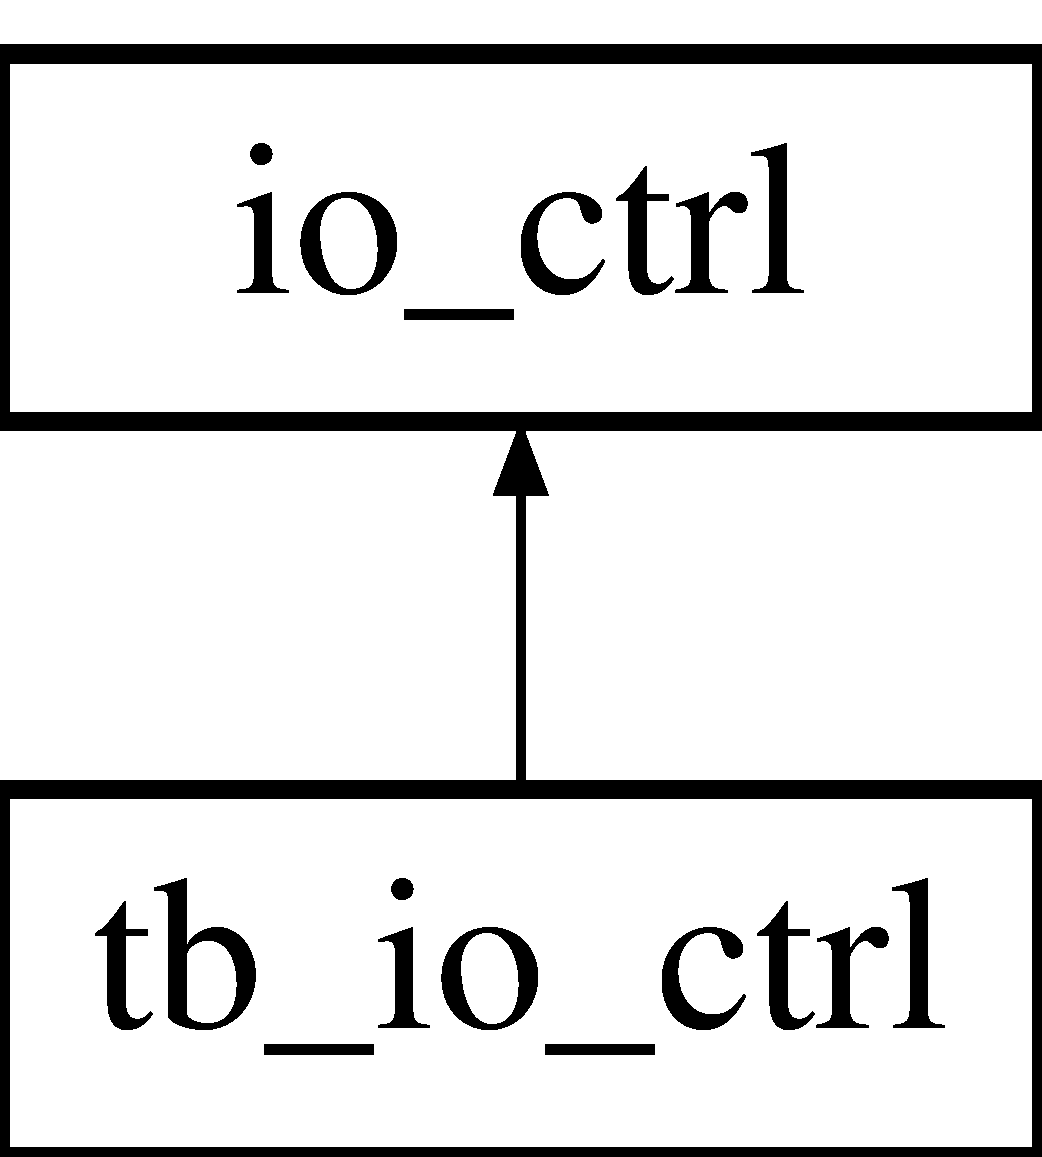
\includegraphics[height=2.000000cm]{classtb__io__ctrl}
\end{center}
\end{figure}
\subsection*{Entities}
\begin{DoxyCompactItemize}
\item 
\hyperlink{classtb__io__ctrl_1_1sim}{sim} architecture
\begin{DoxyCompactList}\small\item\em IO Control Unit Testbench Architecture. \end{DoxyCompactList}\end{DoxyCompactItemize}
\subsection*{Libraries}
 \begin{DoxyCompactItemize}
\item 
\mbox{\Hypertarget{classtb__io__ctrl_ae4f03c286607f3181e16b9aa12d0c6d4}\label{classtb__io__ctrl_ae4f03c286607f3181e16b9aa12d0c6d4}} 
\hyperlink{classtb__io__ctrl_ae4f03c286607f3181e16b9aa12d0c6d4}{I\+E\+EE} 
\end{DoxyCompactItemize}
\subsection*{Use Clauses}
 \begin{DoxyCompactItemize}
\item 
\mbox{\Hypertarget{classtb__io__ctrl_acd03516902501cd1c7296a98e22c6fcb}\label{classtb__io__ctrl_acd03516902501cd1c7296a98e22c6fcb}} 
\hyperlink{classtb__io__ctrl_acd03516902501cd1c7296a98e22c6fcb}{std\+\_\+logic\+\_\+1164}   
\end{DoxyCompactItemize}


\subsection{Detailed Description}
IO Control Unit Testbench Entity. 

The IO Control uniti part of the calculator project. 

The documentation for this class was generated from the following file\+:\begin{DoxyCompactItemize}
\item 
tb/\hyperlink{tb__io__ctrl___8vhd}{tb\+\_\+io\+\_\+ctrl\+\_\+.\+vhd}\end{DoxyCompactItemize}

\chapter{File Documentation}
\hypertarget{tb__io__ctrl___8vhd}{}\section{tb/tb\+\_\+io\+\_\+ctrl\+\_\+.vhd File Reference}
\label{tb__io__ctrl___8vhd}\index{tb/tb\+\_\+io\+\_\+ctrl\+\_\+.\+vhd@{tb/tb\+\_\+io\+\_\+ctrl\+\_\+.\+vhd}}


IO Control Unit Testbench Entity.  


\subsection*{Entities}
\begin{DoxyCompactItemize}
\item 
\hyperlink{classtb__io__ctrl}{tb\+\_\+io\+\_\+ctrl} entity
\begin{DoxyCompactList}\small\item\em IO Control Unit Testbench Entity. \end{DoxyCompactList}\end{DoxyCompactItemize}


\subsection{Detailed Description}
IO Control Unit Testbench Entity. 


\hypertarget{tb__io__ctrl__cfg_8vhd}{}\section{tb/tb\+\_\+io\+\_\+ctrl\+\_\+cfg.vhd File Reference}
\label{tb__io__ctrl__cfg_8vhd}\index{tb/tb\+\_\+io\+\_\+ctrl\+\_\+cfg.\+vhd@{tb/tb\+\_\+io\+\_\+ctrl\+\_\+cfg.\+vhd}}


IO Control Unit Testbench Configuration.  


\subsection*{Configurations}
 \begin{DoxyCompactItemize}
\item 
\mbox{\Hypertarget{tb__io__ctrl__cfg_8vhd_aa44e219cb284ff206422ccc36ce0373b}\label{tb__io__ctrl__cfg_8vhd_aa44e219cb284ff206422ccc36ce0373b}} 
\hyperlink{tb__io__ctrl__cfg_8vhd_aa44e219cb284ff206422ccc36ce0373b}{tb\+\_\+io\+\_\+ctrl\+\_\+cfg}  {\bfseries tb\+\_\+io\+\_\+ctrl}   
\end{DoxyCompactItemize}


\subsection{Detailed Description}
IO Control Unit Testbench Configuration. 


\hypertarget{tb__io__ctrl__sim_8vhd}{}\section{tb/tb\+\_\+io\+\_\+ctrl\+\_\+sim.vhd File Reference}
\label{tb__io__ctrl__sim_8vhd}\index{tb/tb\+\_\+io\+\_\+ctrl\+\_\+sim.\+vhd@{tb/tb\+\_\+io\+\_\+ctrl\+\_\+sim.\+vhd}}


IO Control Unit Testbench Architecture S\+IM.  


\subsection*{Entities}
\begin{DoxyCompactItemize}
\item 
\hyperlink{classtb__io__ctrl_1_1sim}{sim} architecture
\begin{DoxyCompactList}\small\item\em IO Control Unit Testbench Architecture S\+IM. \end{DoxyCompactList}\end{DoxyCompactItemize}


\subsection{Detailed Description}
IO Control Unit Testbench Architecture S\+IM. 


\hypertarget{io__ctrl___8vhd}{}\section{vhdl/io\+\_\+ctrl\+\_\+.vhd File Reference}
\label{io__ctrl___8vhd}\index{vhdl/io\+\_\+ctrl\+\_\+.\+vhd@{vhdl/io\+\_\+ctrl\+\_\+.\+vhd}}


IO Control Unit Entity.  


\subsection*{Entities}
\begin{DoxyCompactItemize}
\item 
\hyperlink{classio__ctrl}{io\+\_\+ctrl} entity
\begin{DoxyCompactList}\small\item\em IO Control Unit Entity. \end{DoxyCompactList}\end{DoxyCompactItemize}


\subsection{Detailed Description}
IO Control Unit Entity. 


\hypertarget{io__ctrl__cfg_8vhd}{}\section{vhdl/io\+\_\+ctrl\+\_\+cfg.vhd File Reference}
\label{io__ctrl__cfg_8vhd}\index{vhdl/io\+\_\+ctrl\+\_\+cfg.\+vhd@{vhdl/io\+\_\+ctrl\+\_\+cfg.\+vhd}}


IO Control Unit Configuration.  


\subsection*{Configurations}
 \begin{DoxyCompactItemize}
\item 
\mbox{\Hypertarget{io__ctrl__cfg_8vhd_ad4882792e0623e919c5c75e031efa056}\label{io__ctrl__cfg_8vhd_ad4882792e0623e919c5c75e031efa056}} 
\hyperlink{io__ctrl__cfg_8vhd_ad4882792e0623e919c5c75e031efa056}{io\+\_\+ctrl\+\_\+rtl\+\_\+cfg}  {\bfseries io\+\_\+ctrl}   
\end{DoxyCompactItemize}


\subsection{Detailed Description}
IO Control Unit Configuration. 


\hypertarget{io__ctrl__rtl_8vhd}{}\section{vhdl/io\+\_\+ctrl\+\_\+rtl.vhd File Reference}
\label{io__ctrl__rtl_8vhd}\index{vhdl/io\+\_\+ctrl\+\_\+rtl.\+vhd@{vhdl/io\+\_\+ctrl\+\_\+rtl.\+vhd}}


IO Control Unit Architecture.  


\subsection*{Entities}
\begin{DoxyCompactItemize}
\item 
\hyperlink{classio__ctrl_1_1rtl}{rtl} architecture
\begin{DoxyCompactList}\small\item\em IO Control Unit Architecture. \end{DoxyCompactList}\end{DoxyCompactItemize}


\subsection{Detailed Description}
IO Control Unit Architecture. 


%--- End generated contents ---

% Index
\backmatter
\newpage
\phantomsection
\clearemptydoublepage
\addcontentsline{toc}{chapter}{Index}
\printindex

\end{document}
